% STEP 1: Choose oneside or twoside. Use the 'draft' option a lot when writing.
\documentclass[english, oneside]{HYgradu}

\usepackage[utf8]{inputenc} % For UTF8 support. Use UTF8 when saving your file.
\usepackage{lmodern} % Font package
\usepackage{textcomp}
\usepackage[pdftex]{color, graphicx} % For pdf output and jpg/png graphics
\usepackage[pdftex, plainpages=false]{hyperref} % For hyperlinks and pdf metadata
\usepackage{fancyhdr} % For nicer page headers
%\usepackage{tikz} % For making vector graphics (hard to learn but powerful)
%\usepackage{wrapfig} % For nice text-wrapping figures (use at own discretion)
\usepackage{amsmath, amssymb} % For better math
\usepackage[round]{natbib} % For bibliography
\usepackage[footnotesize,bf]{caption} % For more control over figure captions
\usepackage{subcaption}

\fussy % Probably not needed but you never know...


% OPTIONAL STEP: Set up properties and metadata for the pdf file that pdfLaTeX makes.
% But you don't really need to do this unless you want to.
\hypersetup{
    bookmarks=true,         % show bookmarks bar first?
    unicode=true,           % to show non-Latin characters in Acrobat’s bookmarks
    pdftoolbar=true,        % show Acrobat’s toolbar?
    pdfmenubar=true,        % show Acrobat’s menu?
    pdffitwindow=false,     % window fit to page when opened
    pdfstartview={FitH},    % fits the width of the page to the window
    pdftitle={},            % title
    pdfauthor={},           % author
    pdfsubject={},          % subject of the document
    pdfcreator={},          % creator of the document
    pdfproducer={pdfLaTeX}, % producer of the document
    pdfkeywords={something} {something else}, % list of keywords for
    pdfnewwindow=true,      % links in new window
    colorlinks=true,        % false: boxed links; true: colored links
    linkcolor=black,        % color of internal links
    citecolor=black,        % color of links to bibliography
    filecolor=magenta,      % color of file links
    urlcolor=cyan           % color of external links
}

% STEP 2:
% Set up all the information for the title page and the abstract form.
% Replace parameters with your information.
\title{Formation of cores by merging supermassive black holes}
\author{Joonas Suortti}
\date{\today}
\level{Master's thesis}
\faculty{Faculty of Whatever}
\department{Department of Something}
\address{PL 42 (Kuvitteellinen katu 1)\\00014 Helsingin yliopisto}
\subject{Your Field}
\prof{prof. Smith}
\censors{prof. Smith}{doc. Smythe}{}
\depositeplace{}
\additionalinformation{}
\numberofpagesinformation{\numberofpages\ pages}
\classification{}
\keywords{Your keywords here}
\quoting{``Bachelor's degrees make pretty good placemats if you get them laminated.'' \\---Jeph Jacques}

\begin{document}

% Generate title page.
\maketitle

% STEP 3:
% Write your abstract (of course you really do this last).
% You can make several abstract pages (if you want it in different languages),
% but you should also then redefine some of the above parameters in the proper
% language as well, in between the abstract definitions.
\begin{abstract}
Abstract goes here.
\end{abstract}

% Place ToC
\mytableofcontents



% -----------------------------------------------------------------------------------
% STEP 4: Write the thesis.
% Your actual text starts here. You shouldn't mess with the code above the line except
% to change the parameters. Removing the abstract and ToC commands will mess up stuff.
\chapter{Introduction}

\chapter{Theory}



\chapter{KETJU}

\textit{Description of basic functionality: what KETJU does, why it's created, basic description of the multiple integration region system.} 

\section{AR-CHAIN}

\textit{Chain forming, force calculations, integration}

\section{GADGET-3}

\textit{Softening, tree-codes, calculations}

\section{Combined Functionality}

\textit{How the AR-CHAIN and GADGET-3 integrators work together: time-step problem, tidal-perturbations, particles moving from one region to another, chain macro-particle}

\subsection{Particle Types}


\section{Black Hole Trajectories}

Since we are trying to determine if merging SMBH binaries form cores in merger remnants, we must make sure that the progenitors' central black holes actually merge in our simulations. This is done by looking at the "Run" simulations, as they contain the locations of the black holes from multiple time steps, and as the "Snapshots" still show both of the SMBHs.

Plotting the positions of the black holes from "Run 3" in coordinates centred on the binary's centre-of-mass during the initial time step gives us figure \ref{figure:run3_traj}. Even by eye, one can clearly see that the orbit of the black hole with a smaller mass becomes smaller and smaller as the binary moves further away from its initial position. While this doesn't explicitly tell us that the black holes merge into each other, it does indicate the existence of a hardening process in the binary. Similar figures to figure \ref{figure:run3_traj} from all four "Runs" can be found in the appendix (figure \ref{figure:all_traj}).

\begin{figure}[h]
	\centering	
	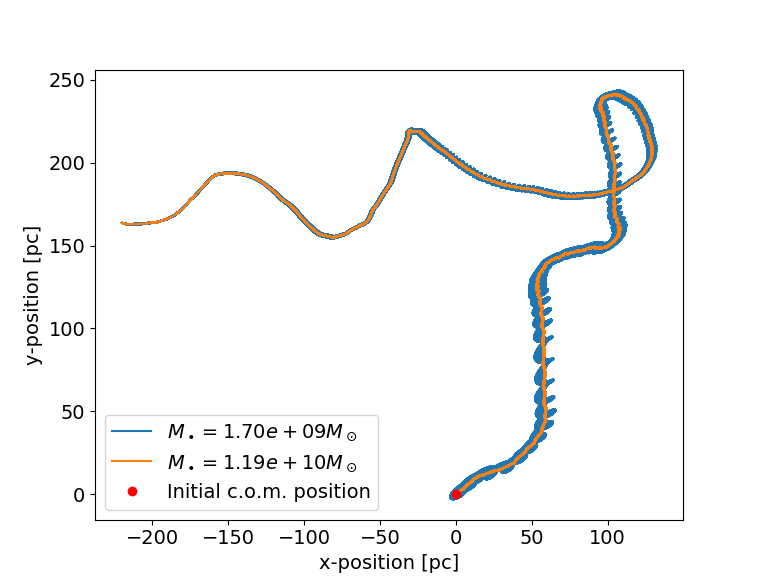
\includegraphics[width=0.7\textwidth]{Run3_Trajectory.png}	
	\caption{The trajectories of the black holes during "Run 3". The coordinates are centred on the initial location of the centre-of-mass of the binary black hole. The orange and blue lines show the paths taken by the smaller and larger black holes respectively. Both paths show clear spiral patterns which become smaller and smaller as the simulation proceeds. The paths end at the location where the black holes merge, i.e. where the distance between them is $\lesssim 100 R_s$ ($R_s$ is the Schwarzschild radius).}
	\label{figure:run3_traj}
\end{figure}

\begin{figure}[h]
	\centering
	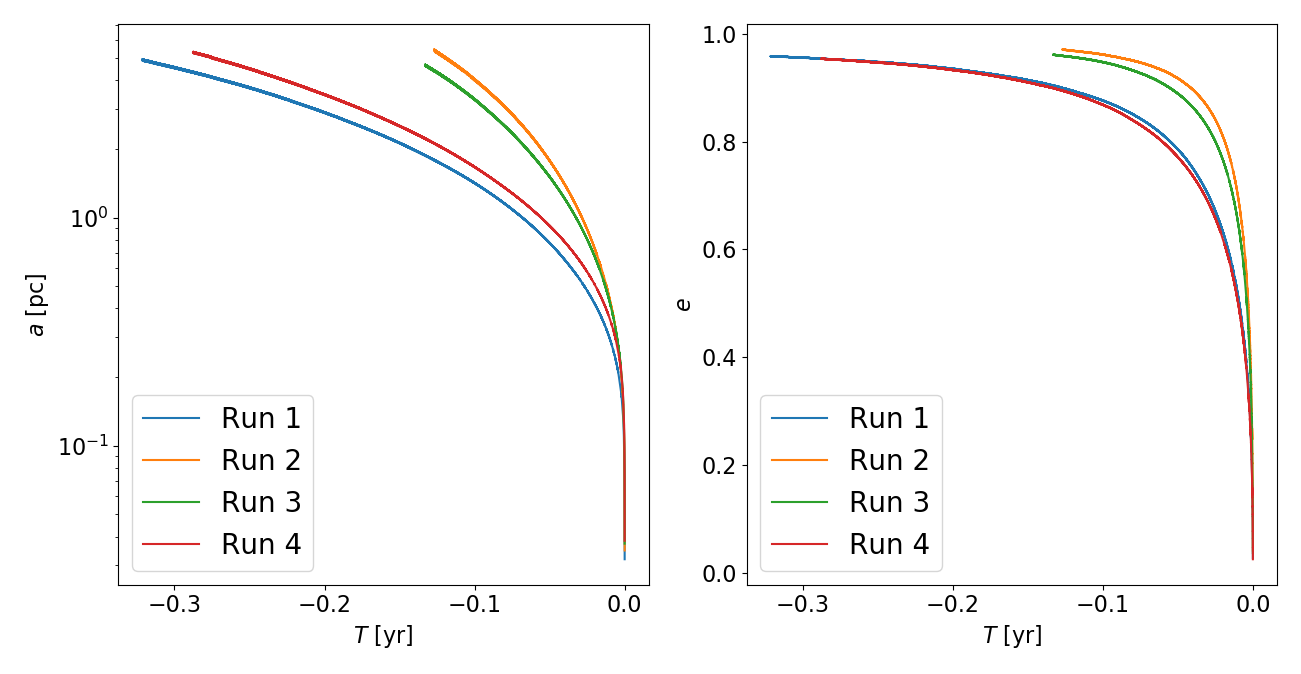
\includegraphics[width=\textwidth]{semi_major_and_ecc.png}
	\caption{The semi-major axes (left) and eccentricities (right) of the black hole systems in the simulations "Runs 1"-"Run-4" as a function of time. The zero position on the x-axis corresponds to the point in simulation time, where the black hole merging event occurs.}
	\label{figure:semi_and_ecc}
\end{figure}

%Figure \ref{figure:semi_and_ecc} shows the time evolution of the semi-major axis $a$ and the eccentricity $e$ of the binary from every run. The behaviour of both $a$ and $e$ indicate that the binary does actually merge, as the orbits go from highly eccentric to almost circular, and as $a$ declines exponentially.

The most likely obstacle for the complete merging of the binary black holes is the so-called final-parsec problem; where, due to the lack of stellar material that can be ejected during the three-body scattering phase, the hardening of the binary stops when the separation between the two black holes is $\sim 1 \mathrm{pc}$. This is assumed to happen since, not only is the binary constantly ejecting the finite amount of stars inside the loss-cone (defined in section 2), but the loss cone itself is becoming smaller due to the contracting binary orbit.

Figure \ref{figure:semi_and_ecc} shows the time evolution of both the semi-major axis and the eccentricity of the binary orbits from all of the simulation runs. Interestingly enough the semi-major axes of all of the binaries go far below single parsec scales, meaning that the final-parsec problem doesn't seem to play a part in the simulations. This implies that, there exists some loss-cone refill mechanism which allows the binary to eject more stellar material than what initially exists inside the loss cone.



\chapter{Merger Simulations Using KETJU}

In this chapter I study the formation of cored galaxies through galaxy mergers by analysing results from KETJU simulations by \cite{Rantala2018}. The merger progenitor galaxies in these simulations contain central supermassive black holes. During the merger event, the SMBHs form a hard binary, a likely source for the observed cores, as it can eject stars from the galactic centre through complex three-body interactions. Here I determine if there is a connection between the binary SMBH and the existence of a core deficient in light, and if the simulated KETJU results agree with observations.


\section{Simulation Details}

The simulations done by \cite{Rantala2018} include seven different mergers of two identical galaxies. The merger progenitor galaxies used in the different simulations (named BH-0 - BH-6) are comprised of stellar and dark matter particles, with the different particle types having identical masses. They are gas free (i.e. the simulations describe so-called "dry" mergers), and most of them contain an SMBH at their centre.

The progenitors' central SMBHs are simply modelled as point masses, located at the origin of the galaxy's internal coordinate system; while the stellar and dark matter particles are distributed according to the spherically symmetric Dehnen density-potential model \citep{Dehnen1993}:
\begin{equation}
\rho(r) = \frac{(3-\gamma)M}{4\pi} \frac{a}{r^\gamma (r+a)^{4-\gamma}}, \label{eq:dehnen_density}
\end{equation}
\begin{equation}
\phi(r) = \frac{GM}{a} \times 
\begin{cases}
	-\frac{1}{2-\gamma} \left[ 1 - \left( \frac{r}{r+a} \right)^{2-\gamma} \right] & \; \gamma \neq 2 \\
	\ln \frac{r}{r+a}	 & \; \gamma = 2
\end{cases},
\label{eq:dehnen_potential}
\end{equation}
where $M$ is the total mass, $a$ is a scaling radius, and $\gamma$ is the central slope of the profile. For stellar particles $\gamma = 3/2$, while for the dark matter particles $\gamma = 1$. 

Using the Dehnen density-potential model, the positions of the different particles are determined through the cumulative mass profile:
\begin{equation}
M(r) = 4\pi \int^r_0 \rho(r)r^2 \;dr = M \left( \frac{r}{r+a} \right)^{3-\gamma}, \label{eq:cumulative_mass}
\end{equation}
where $\rho(r)$ is the density profile from equation \ref{eq:dehnen_density}. Once the positions of the particles are known, their velocities can also be determined using the Eddington's formula \citep{BinneyTremaine}, which gives the following distribution function for the different particles in the position-velocity phase-space:
\begin{equation}
f_i(\varepsilon) = \frac{1}{\sqrt{8}\pi^2} \int^{\Phi_T = \varepsilon}_{\Phi_T = 0} \frac{d^2\rho_i}{d\Phi^2_T}
\frac{d\Phi_T}{\sqrt{\varepsilon - \Phi_T}}, \label{eq:eddington_form}
\end{equation}
where $\rho_i$ is the density profile from equation \ref{eq:dehnen_density} for the particle in question, $\Phi_T$ is the total gravitational potential, and $\varepsilon$ is the relative energy:
\begin{equation}
\varepsilon = -\Phi_T + \Phi_0 - \frac{1}{2} v^2,
\end{equation}
where $v$ is the velocity of the particle and $\Phi_0$ is a chosen zero point for the potential. This zero point is usually chosen so that, $f > 0$ for $\varepsilon > 0$, and $f = 0$ for $\varepsilon \leq 0$. In the case of the analysed simulations $\Phi_0 = 0$, as the modelled galaxies are isolated and extend to infinity.

The physical parameters needed for generating the progenitor galaxies using equations \ref{eq:cumulative_mass} and \ref{eq:eddington_form} are given in table \ref{table:properties} under "Common physical properties", and, as name implies, are identical across all of the progenitors used in the simulations. While the uses for the number of stellar and dark matter particles, and the stellar and dark matter masses, are self-explanatory; the effective radius $R_e$ and dark matter fraction inside the half-mass radius $f_\mathrm{DM}(r_{1/2})$ are used for determining the scaling radius $a$ with the equations:
\begin{equation}
a_\star = r_{1/2}(2^{1/(3-\gamma)}-1); \quad r_{1/2} \approx 4/3 R_e,
\end{equation}
and
\begin{equation}
a_\mathrm{DM} \approx \frac{4}{3} \left[ \sqrt{\frac{2M_\mathrm{DM}}{M_\star} \left( \frac{1}{f_\mathrm{DM}(r_{1/2})} - 1 \right)} -1 \right] R_e,
\end{equation}
, for the stellar and dark matter particle profiles respectively. The values for the common properties are motivated by observations and dynamical simulations of NGC 1600 \citep{Rantala2018}, an early-type cored galaxy with a large core radius and a central supermassive black hole with a mass of $\sim 1.7 \times 10^{10} M_\odot$ \cite{Thomas2016}.

\begin{table}
	\begin{center}
		\begin{tabular}{| c c c c c c c |}
		\hline
		\multicolumn{7}{|c|}{Common physical properties} \\
		\hline
		$M_\star$ & $R_e$ & $M_\mathrm{DM}$ & $f_\mathrm{DM}(r_{1/2})$ & $N_\star$ & $N_\mathrm{DM}$ & \\
		$4.15$ & $7$ & $7.5$ & $0.25$ & $4.15 \times 10^6$ & $1.0 \times 10^7$ & \\
		\hline
		\hline
		\multicolumn{7}{|c|}{$M_\bullet$} \\
		\hline
		BH-0 & BH-1 & BH-2 & BH-3 & BH-4 & BH-5 & BH-6 \\
		- & $0.85$ & $1.7$ & $3.4$ & $5.1$ & $6.8$ & $7.5$ \\
		\hline
		\end{tabular}
	\end{center}
	\caption{Physical properties of the different progenitors used in the simulations by \cite{Rantala2018}. \\
	$M_\star$: Stellar mass $[\times 10^{11} M_\odot]$ \\
	$R_e$: Effective radius $[\mathrm{kpc}]$ \\
	$M_\mathrm{DM}$: Dark matter halo mass $[\times 10^{13} M_\odot]$\\
	$f_\mathrm{DM}(r_{1/2})$: The fraction of dark matter mass from the total mass inside the effective radius \\
	$N_\star$: Number of stellar particles \\
	$N_\mathrm{DM}$: Number of dark matter particles \\
	$M_\bullet$: Central SMBH Mass $[\times 10^9 M_\odot]$}
	\label{table:properties}
\end{table}

Table \ref{table:properties} also shows the masses of the central SMBHs in each of the seven progenitor galaxies. The mass of the central SMBH is the only physical property that changes from one progenitor to another. Six of the progenitor galaxies (BH-1 - BH-6) contain central supermassive black holes, with the SMBH masses varying from $8.5 \times 10^8 M_\odot$ to $8.5 \times 10^9 M_\odot$, where a merged binary of the largest SMBHs is equivalent in mass to the central SMBH in NGC 1600. The seventh progenitor (BH-0) does not contain an SMBH in its centre, and is included simply for the sake of comparison.

The simulations themselves comprise of seven mergers of two identical progenitor galaxies from table \ref{table:properties}, where the galaxies are merged on a nearly parabolic orbit with an initial separation of $d = 30 \mathrm{kpc}$. According to \cite{Rantala2018}, this kind of orbit makes the approach of the galaxies swift, and causes the stellar cusps to merge before $t \sim 300 \mathrm{Myr}$.

The simulation data, that I will be analysing, comes in the form of a snapshot of the merger remnant at the simulation time of $\sim 2 \mathrm{Gyr}$. At this point the progenitor galaxies have merged into a single merger remnant galaxy, which contains an SMBH binary in its centre. The analysed snapshots contain the positions, velocities and masses of every particle; be they stellar particles, dark matter particles or black holes.

\section{Core Size Measurements}

In order to check if a galaxy is cored or not, I calculate its surface brightness profile and check if the galaxy contains surface brightness deficiencies near its centre.

The surface brightness profiles are calculated from the merger remnant snapshots by: changing the coordinate system to centre-of-mass coordinates, projecting the stellar particles onto a 2D plane, and calculating the mass inside logarithmically spaced radial bins to get a radial surface mass density profile. The aforementioned calculations are repeated 100 times from random viewing angles, which results in 100 slightly different density profile projections. These profiles are then averaged azimuthally, which results in a smooth surface mass density profile, that can then be turned into a surface brightness profile by assuming some mass-to-light ratio for the stellar particles \citep{Rantala2018}. However, as the only properties that the stellar particles have in the snapshot are: their position and velocity at a singular point in time, as well as a mass that is identical to the mass of every other stellar particle; it is not possible to make valid, physically accurate, assumptions on their specific mass-to-light ratios. For this reason, a constant mass-to-light ratio of $M/L = 4$ is used, which is equivalent to the ratio derived from dynamical modelling of NGC 1600 by \cite{Thomas2016}.

Figure \ref{figure:surface_brightness} shows example surface brightness profiles for every simulated merger remnant. Looking at the different curves, one can clearly see that the presence of central SMBHs in the merger progenitors causes some kind of brightness deficiency near the merger remnant's centre. Not only that, the larger the mass of the central black holes, the larger the surface brightness deficiencies are.

\begin{figure}[h]
	\centering
	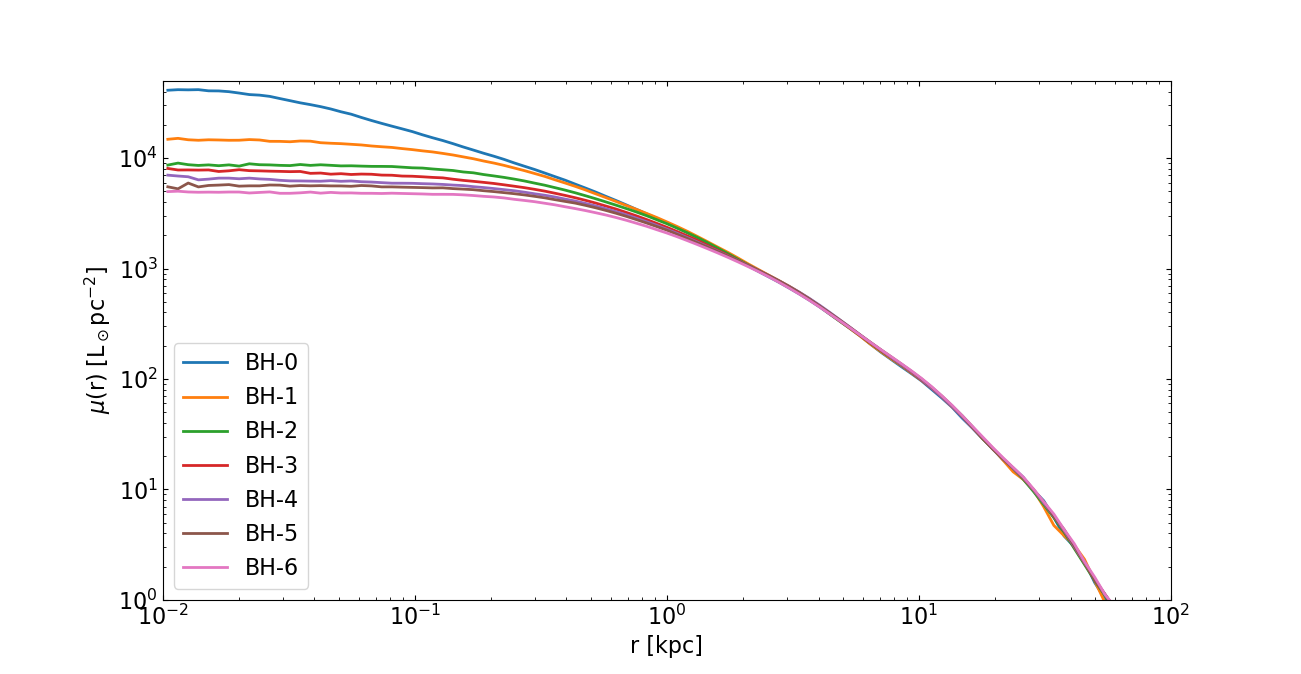
\includegraphics[width=\textwidth]{SurfaceBrightnessProfiles.png}
	\caption{Surface brightness profiles from every snapshot. These were calculated by dividing the simulated galaxy remnants into 100 radial logarithmic bins, and averaging the surface brightness inside the bins through 100 random viewing angles. The luminosity of the particles was estimated by assuming a mass-to-light ratio of $M/L = 4$.}
	\label{figure:surface_brightness}
\end{figure}

The deficiencies found in the surface brightness profiles reveal the presence of cores; however, determining the precise sizes of the cores require us to find the exact locations where the deviations from the expected power-law profile start. This can be done by fitting the derived brightness profile with a model that is a combination of two power laws: a shallow inner power-law, and a steeper outer power-law. The radius at which the power laws shift, i.e. the break radius $r_b$, is defined as the radius of the core. 

There are two commonly used options for modelling the surface brightness profiles. The first one is the core-Sérsic profile \citep{Graham2003}, which can be expressed using the following equation:
\begin{equation}
\mu(r) = \mu' \left[ 1 + \left( \frac{r_b}{r} \right)^\alpha \right]^{\gamma / \alpha} \exp \left\lbrace -b_n \left[ \left( r^\alpha + r_b^\alpha \right) / r_e^\alpha \right]^{1/(\alpha n)} \right\rbrace, \label{eq:core-sersic}
\end{equation}
where $r_b$ is the break radius, $\gamma$ is the logarithmic slope of the inner power-law, $\alpha$ controls the sharpness of the transition between the two power-laws, $r_e$ and $n$ are the effective half-mass radius and the Sérsic index of the outer power-law, and the normalization factor $\mu'$ is defined by:
\begin{equation}
\mu' = \mu_b 2^{-\gamma/\alpha} \exp \left[ b_n \left( 2^{(1/\alpha)} r_b/r_e \right)^{1/n} \right], 
\label{eq:mu_dot}
\end{equation}
where $\mu_b$ is the surface brightness at the break radius. 

The second option is to use the so called Nuker profile \citep{Lauer1995}:
\begin{equation}
\mu(r) = 2^{(\beta - \gamma) / \alpha} \mu_b \left( \frac{r_b}{r} \right)^\gamma \left[ 1 + \left( \frac{r}{r_b} \right)^\alpha \right]^{(\gamma - \beta)/\alpha},
\label{eq:nuker}
\end{equation}
where $r_b$ is once again the break radius, $\mu_b$ is the surface brightness at the break radius, $\beta$ and $\gamma$ are the logarithmic slopes of the power-laws inside and outside of the break radius respectively, and $\alpha$ is the sharpness of the transition between the two slopes.

\begin{figure}[h]
	\centering
	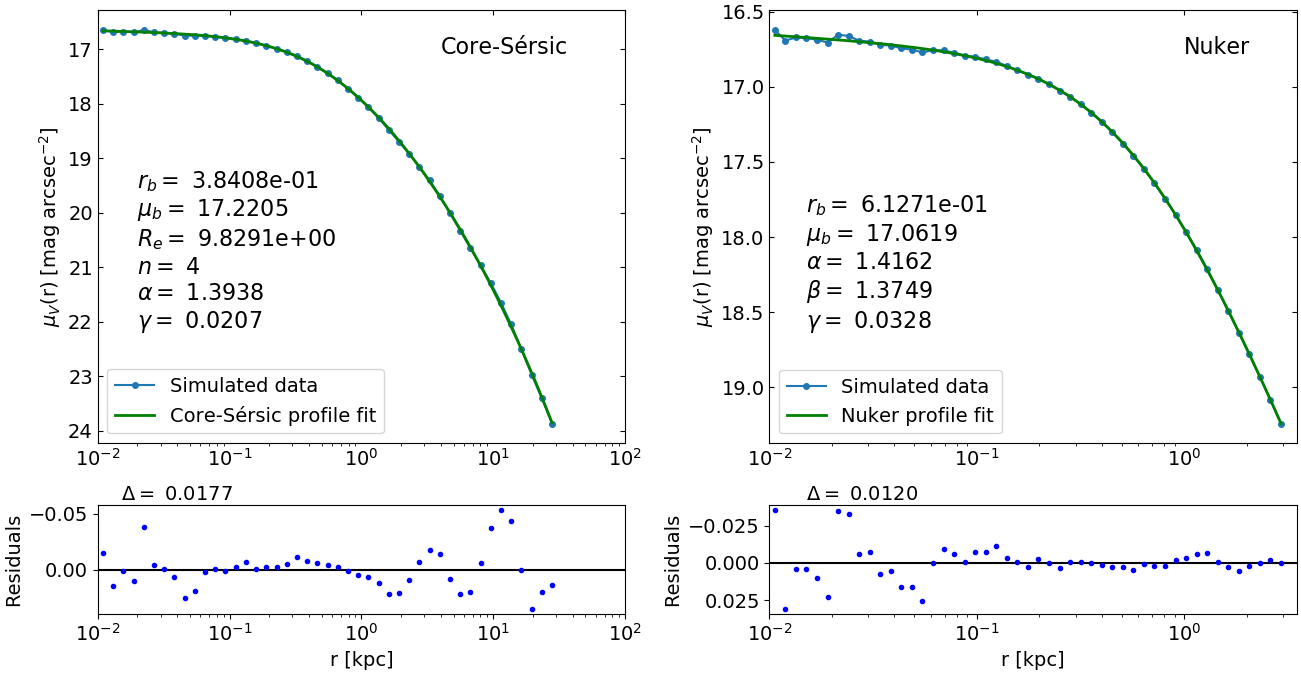
\includegraphics[width=\textwidth]{core_nuker_fits.png}
	\caption{Core-Sérsic and Nuker profile fits of surface brightness profiles calculated from Snapshot 3 (left and top-right figures). The best fit parameters are written on the figures and are in the same units as the axes (i.e. $r_b$ and $R_e$ in kilo-parsecs, and $\mu_b$ in V-band magnitudes per arc-second squared). The relative residuals of the fits are plotted under their respective figures. The delta describes the root-mean-square of the residuals.}
	\label{figure:core_nuker}
\end{figure}

We calculate the core radii of the merger remnants by using the "Levenberg-Marquardt" fitting algorithm to fit both the core-Sérsic model and the Nuker model to the remnant's surface brightness profile. Figure \ref{figure:core_nuker} shows a comparison of the resulting fits for the BH-3 merger (refer to table \ref{table:properties}), while figures \ref{figure:all_core} and \ref{figure:all_nuker}, located in the appendix, show the fits for every remnant that contains SMBH binaries. The values of the best-fit parameters are written on the figures.

The residuals of the fits are comparable to those seen in fits of observed surface brightness profiles ($\Delta \approx 0.02 \; \mathrm{mag \; arcsec^{-2}}$ \citep{Dullo2012}). This implies that the fits are accurate, however, some parts of the fits do seem to show systematically larger residual scatter than other. Most of the fits, especially the Nuker fits, have large residual scatter near the centre of the merger remnant. This means that the central regions do not contain smooth luminosity profiles, which implies that, close to the centres of the galaxies, the stellar particles themselves are not distributed as smoothly as in other other regions. Areas of seemingly randomly placed stellar particles could be attributed to the ejection of the stellar material by an SMBH binary; as it is mainly the velocity, not the location, of the stellar particles plays a part in determining if the particle is ejected.  

All of the core-Sérsic fits also show a peak in the size of the residuals at around $\sim 10 \mathrm{kpc}$. While this residual property is probably just the result of using mostly identical initial conditions, the fact that it appears in the results of every simulation, shows that, even though the merging SMBHs cause large changes in the central regions of the merger remnant, they leave the outer regions mostly unaffected.

Before studying the break radii, it is useful to also analyse some of the other fit parameters, since they might provide some interesting information about the mergers. Figure \ref{figure:all_core} shows that the central SMBH binary mass does not seem to have a systematic effect on the merger remnants' effective radii. Seeing as the central luminosity deficit grows with the binary's mass, one would assume that, in order to account for the larger amount of missing light, the effective radius would follow suit. However, as this is not the case, one may conclude that; either the larger loss in of total luminosity of the remnant already accounts for the larger luminosity deficit in the centre; or, due to some computational error, the effective radii in question do not provide physically accurate results.

... $\alpha$ analysis? ...

Figures \ref{figure:all_core} and \ref{figure:all_nuker} show that the core radius estimate depends quite strongly on the used model. However, which model is better for estimating the size of the core is still a matter of debate \citep{Lauer2007, Dullo2012}. While the RMS of the relative residuals seems to be consistently (although just marginally) smaller for the Nuker model, when compared to the RMS for the core-Sérsic model (compare figures \ref{figure:all_core} and \ref{figure:all_nuker}), one also has to take into account that in the Nuker model the best-fit value for $r_b$ is strongly dependent on the fitting range \citep{Graham2003Nuker}. Furthermore, as stated by \cite{Rantala2018}, in order to get sensible values for all of the model parameters (e.g. $\alpha \lesssim 1$ might even prevent the model from describing the profile as a combination of two power-laws), the fitting range of the Nuker model has to be narrowed down closer to the galactic centre. This, when combined with the parameters' high dependence of the fitting range, brings into question the sensibility of using the Nuker model for core radius estimation.

One could also estimate the size of the core without model fitting by calculating the so-called "cusp radius" $r_\gamma$, i.e. the distance from the galactic centre at which the logarithmic slope of the surface brightness profile $\gamma' = -1/2$ \citep{Carollo1997, Lauer2007Cusp}. Because the cusp radius $r_\gamma$ also provides an estimate for the location where the inner power-law of the profile changes into the outer power-law, it equates to the core radius. 

We calculate $r_\gamma$ for all of the merger remnants with SMBH binaries (BH-1 - BH-6 mergers) by calculating the gradient of the surface brightness profiles, and then using a "Nelder-Mead" minimization algorithm to find the radius, at which the gradient gets the value $-1/2$. 

\begin{figure}[h]
	\centering
	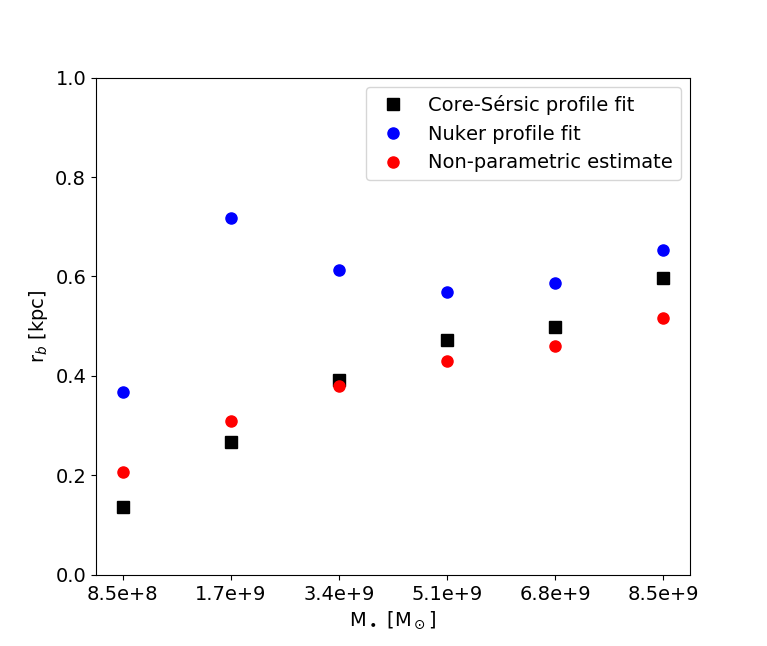
\includegraphics[width=0.7\textwidth]{rb_mass_relation.png}
	\caption{Comparison of the core radii of the merger remnants, gained through three different methods: Core-Sérsic profile fitting (black squares), Nuker profile fitting (blue circles) and  finding the "cusp radius" (red circles). The x-axis shows the masses of the central SMBHs of the merger progenitors.}
	\label{figure:radii_comparison}
\end{figure}

Figure \ref{figure:radii_comparison} compares the core radius estimates from each of the three methods for every simulated merger remnant. The break radii from the Nuker fits are consistently larger than the other core radius estimates. They also have, in general, the largest deviations from the other core radius estimates. Nevertheless, when not accounting for a few of the Nuker break radii, a clear trend of the size of the core growing with the merger progenitors' central SMBH masses can be seen.

The size of the core being dependent on the mass of the central SMBH binary is clear evidence towards the cores being formed through a scouring process by the binary black holes. Binaries with larger masses have a larger gravitational sphere-of-influence, which naturally leads to further ejection of stellar particles orbiting farther away from the galactic centre...



\section{Velocity Anisotropy}

%\begin{figure}[h]
%	\centering
%	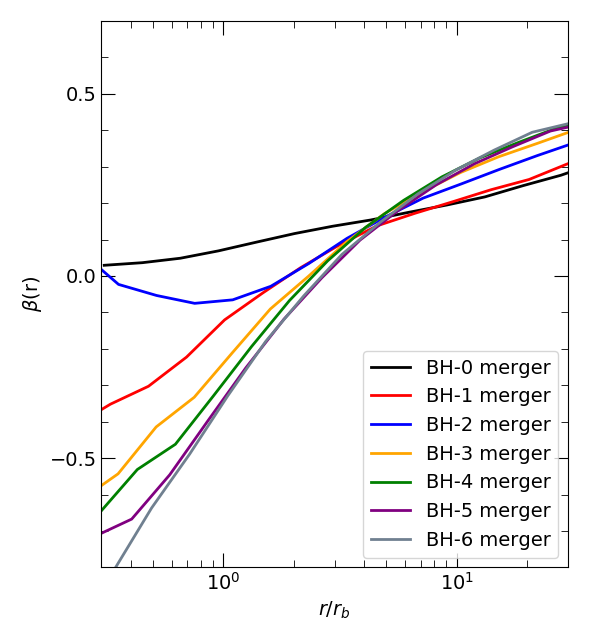
\includegraphics[width=0.9\textwidth]{beta.png}
%	\caption{Velocity anisotropy (beta) profiles of the simulated merger remnants with central black holes.}
%\end{figure}

Another way to find out that a galaxy has formed a core through core scouring by binary black holes, is to study its velocity anisotropy profile defined in \cite{BinneyTremaine}:
\begin{equation}
\beta(r) = 1 - \frac{\sigma_\theta^2 - \sigma_\phi^2}{2\sigma_r^2} = 1 - \frac{\sigma_t^2}{\sigma_r^2}, \label{eq:beta}
\end{equation}
where $\sigma_\theta$, $\sigma_\phi$ and $\sigma_r$ are velocity dispersions in the spherical coordinates, and $\sigma_t = \sqrt{(\sigma_\theta^2 + \sigma_\phi^2) / 2}$ is the tangential velocity dispersion. This $\beta$ parameter describes the ratio of tangential velocity dispersion to radial velocity dispersion, and as such, gives information about the nature of the stellar orbits around the black hole binary. A negative value for $\beta$ shows an abundance of tangential orbits, where as a positive $\beta$ an abundance of radial orbits. 

Figure \ref{figure:beta_no_rb} shows $\beta$-profiles calculated from all of the merger remnant snapshots using equation \ref{eq:beta}. According to the profiles, the outer areas of the remnants are dominated by radial orbits, while the majority of orbits near the centre are tangential.

\begin{figure}[h]
	\centering
	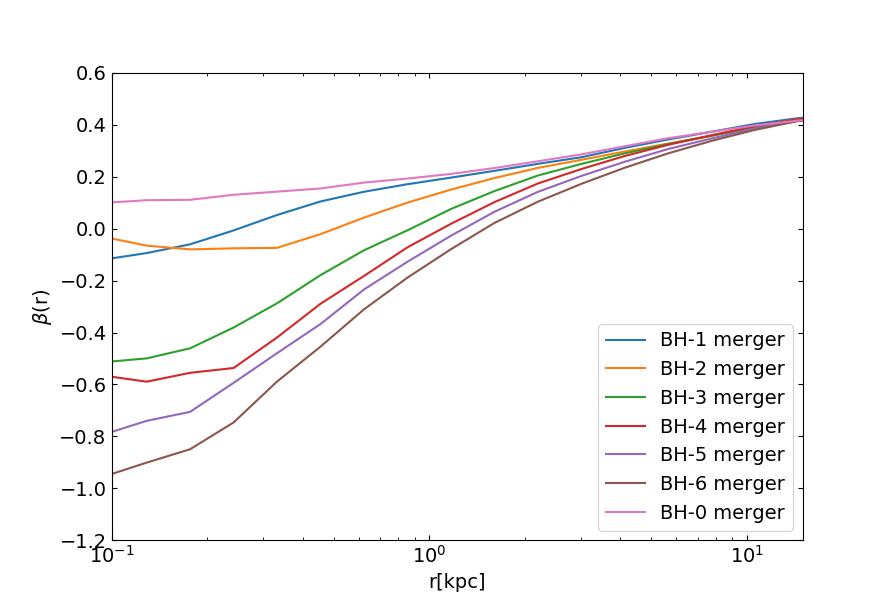
\includegraphics[width=0.9\textwidth]{beta_no_rb.png}
	\caption{Velocity anisotropy (beta) profiles for every simulated merger remnant.}
	\label{figure:beta_no_rb}
\end{figure}

As the progenitors used in the simulations contained $\beta$-profiles which had a constant value of $\beta = 0$, an area with negative $\beta$ in the merger remnant would imply that the stars on radial orbits have been ejected from the system. It has been shown that hardening black hole binaries can eject stars on highly radial orbits from the galactic core, which results in the central region becoming dominated by mostly tangential orbits (and thus a negative $\beta$), while the ejected stars can, in turn, cause the outer orbits to become more radial \citep{Quinlan1997, Milosavljevic2001, Thomas2014}. 

This could certainly be the reason behind the shapes if the central regions in the $\beta$-profiles seen in figure \ref{figure:beta_no_rb}, as it clearly shows that the presence of an SMBH binary has an effect on the profiles' shape. Not only does the slope of the profile steepen as the mass of the SMBH binary grown; but the only merger with a profile, completely dominated by the radial velocity dispersion, is the one without a central binary. 

The properties seen in the profiles also make sense in the context of ejection of stellar particles by hardening black hole binaries. The larger the mass of the SMBH biary is, the larger its gravitational sphere-of-influence, which results in more of the radially orbiting stellar particles being ejected.

\begin{figure}
	\centering
	\begin{subfigure}[b]{0.39\textwidth}
		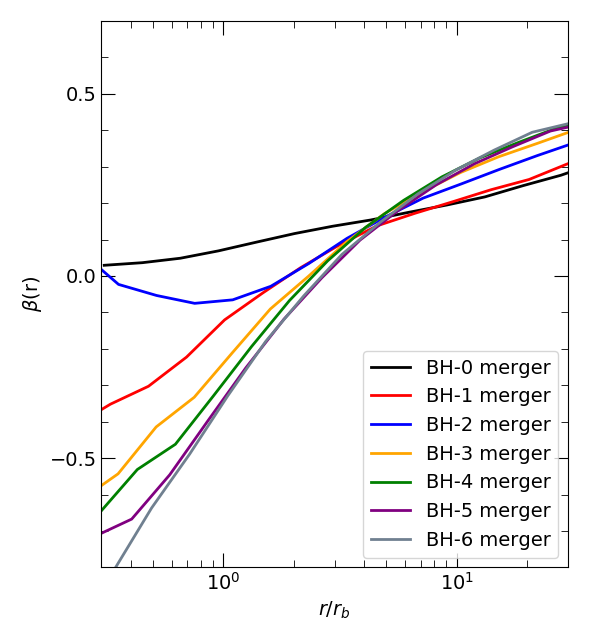
\includegraphics[width=\textwidth]{beta.png}	
		\caption{Simulated merger remnants}
	\end{subfigure}
	\begin{subfigure}[b]{0.60\textwidth}
		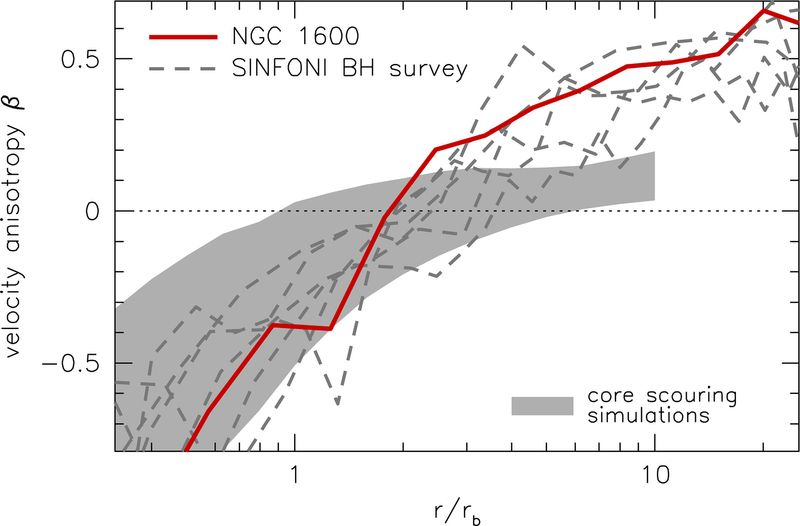
\includegraphics[width=\textwidth]{thomas2016.jpg}
		\caption{NGC 1600}
	\end{subfigure}
	\caption{(a): $\beta$-profiles of the simulated merger remnants as a function of distance from the centre, relative to the break radius. (b): $\beta$-profile of NGC 1600, alongside profiles of galaxies from the SINFONI black hole survey (references), and the range of anisotropies found in N-body simulations of the core scouring mechanism \citep{Thomas2016}.}
	\label{figure:beta_NGC1600_Simul}
\end{figure}

Figure \ref{figure:beta_NGC1600_Simul} shows both the $\beta$-profile from NGC 1600, as well as the profiles from the simulated merger remnants, relative to the core radius of the respective galaxy. Even by eye, it can be seen that the $\beta$-profiles from both simulations and NGC 1600 are similar to each other (not counting the profile for the BH-2 merger). However, the profile for NGC 1600 does seem to be somewhat steeper than any of the ones from the simulated galaxies.

According to \cite{Rantala2018}, it is likely that the higher steepness of the profile, seen in observed galaxies, is due to the fact that the simulations only comprise a single generation of, completely isotropic ($\beta = 0$), mergers. Most actual cored galaxies are the result of multiple merger events, every one of which forms a merger remnant with a steeper profile than what the progenitors had...

\section{Line-of-Sight Kinematics}

In order to make sure that the KETJU simulations produce results equivalent to observations, I analyse the line-of-sight (LOS) kinematics of the simulated merger remnants. The analysis is focused on four different LOS velocity distribution properties: the average LOS velocity $V_\mathrm{avg}$, the velocity dispersion $\sigma$, and the $h_3$ and $h_4$ parameters which correspond to the skewness and the kurtosis of the distribution respectively. The distribution from which these properties are calculated is defined as the following modified Gaussian function \citep{VanDerMarel1993, Bender1994}:
\begin{equation}
f(v) = I_0 e^{-\gamma^2/2}(1 + h_3 H_3(y) + h_4 H_4(y)), \label{eq:mod_gaussian}
\end{equation} 
where $I_0$ is a normalization constant, $\gamma$ is the central slope of the particle density profile, $y = (v - V_\mathrm{avg})/\sigma$, and $H_3$ and $H_4$ are the third and fourth order Hermite polynomials respectively:
\begin{eqnarray}
H_3(y) = \left(2\sqrt{2}y^3 - 3\sqrt{2}y\right) / \sqrt{6}, \\
H_4(y) = \left(4y^4 - 12y^2 + 3 \right) / \sqrt{24}.
\end{eqnarray}

In order to calculate the above properties, we first define the "line-of-sight" as the intermediate axis of the merger remnants, and orient the remnant accordingly using the inertia tensor. Next, we divide a 2D line-of-sight projection of the remnant into "spaxels" (or simply bins), using the voronoi tessellation algorithm \citep{Cappellari2003}. The shape and size of the spaxels are determined so that each one contains the same signal-to-noise ratio, which in our simulated case is defined as the number of stellar particles. The LOS-velocities inside the spaxels are then made into a histogram, into which we fit the modified Gaussian function described in equation \ref{eq:mod_gaussian}. This gives us the values of the LOS-velocity distribution parameters: $V_\mathrm{avg}$, $\sigma$, $h_3$ and $h_4$ for the spaxel in question. Finally, the values of the spaxels can be plotted, giving us 2D voronoi binned maps of all of the four parameters.

Figure \ref{figure:IFU-maps} shows the voronoi binned 2D maps of the four LOS velocity distribution parameters for BH-0 merger and BH-6 merger. The contours denote the merger remnants' flux isophotes, and have a spacing of one magnitude. Similar maps for every merger remnant can be seen in figures \ref{figure:all_voronoi_1} and \ref{figure:all_voronoi_2} in the appendix.

The IFU maps in figures \ref{figure:all_voronoi_1} and \ref{figure:all_voronoi_2} show that the line-of-sight kinematics of the simulated merger remnants are far from isotropic, with some of the maps from simulations with larger central SMBHs showcasing counter-rotating central regions or "kinematically distinct cores" (KDC). These features, alongside the relatively low average LOS-velocities, are found in galaxies called "slow rotators" \citep{Emsellem2007}. Slow rotator galaxies are early type galaxies which are assumed to have been formed through gas-poor "dry" mergers \citep{Emsellem2007, Cappellari2007}; processes not unlike the ones simulated in our simulations. As such, the merger remnants being slow rotators is a somewhat expected result. However, it also implies that the KETJU simulations do produce physically accurate results.

\begin{figure}
	\centering
	\begin{subfigure}[b]{0.49\textwidth}
		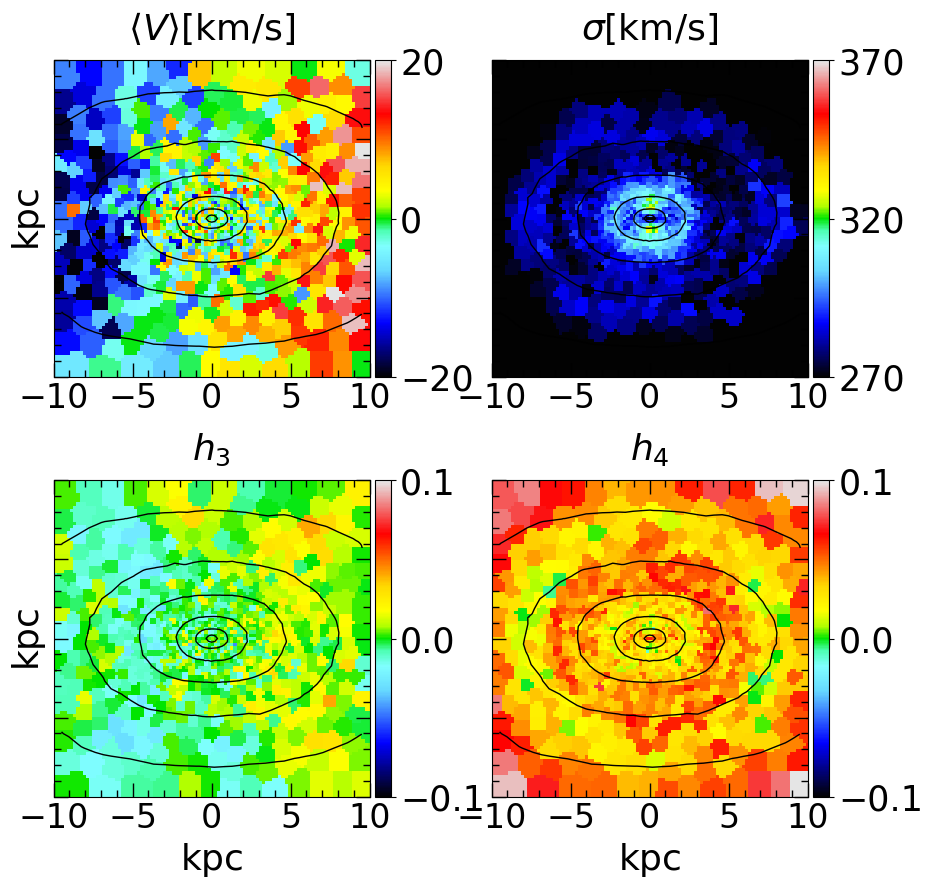
\includegraphics[width=\textwidth]{BH_0.png}
		\caption{BH-1 merger remnant}
	\end{subfigure}
	\begin{subfigure}[b]{0.49\textwidth}
		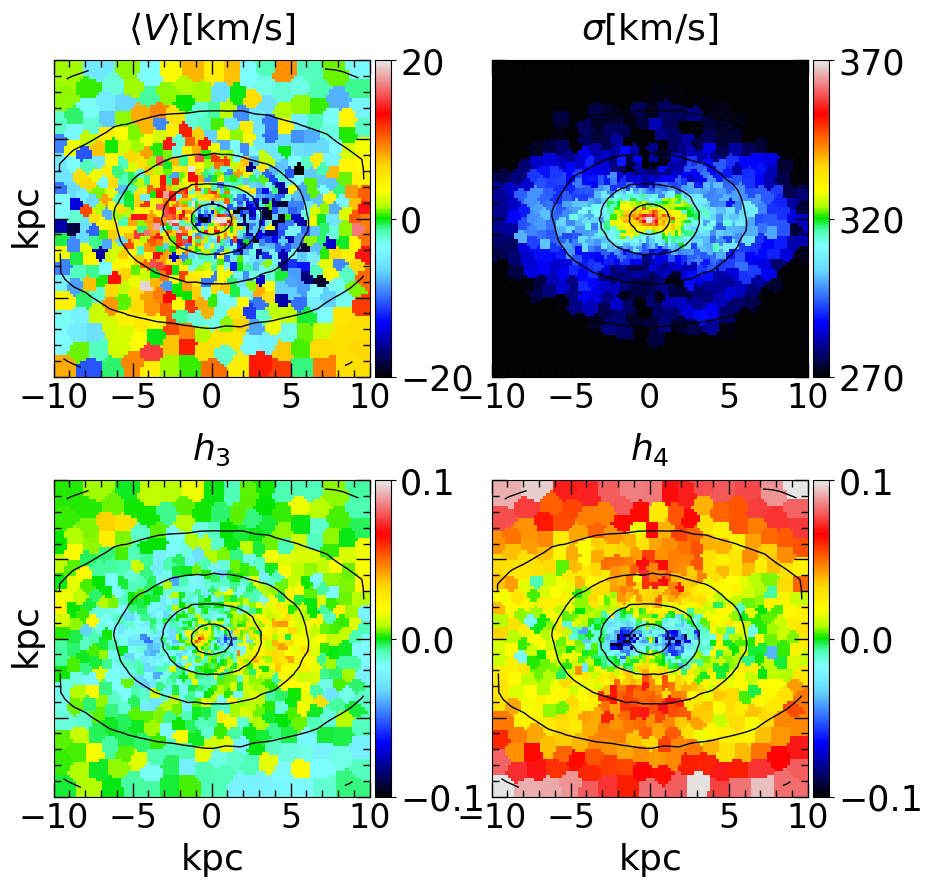
\includegraphics[width=\textwidth]{BH_6.png}
		\caption{BH-6 merger remnant}
	\end{subfigure}
	\begin{subfigure}[b]{0.49\textwidth}
		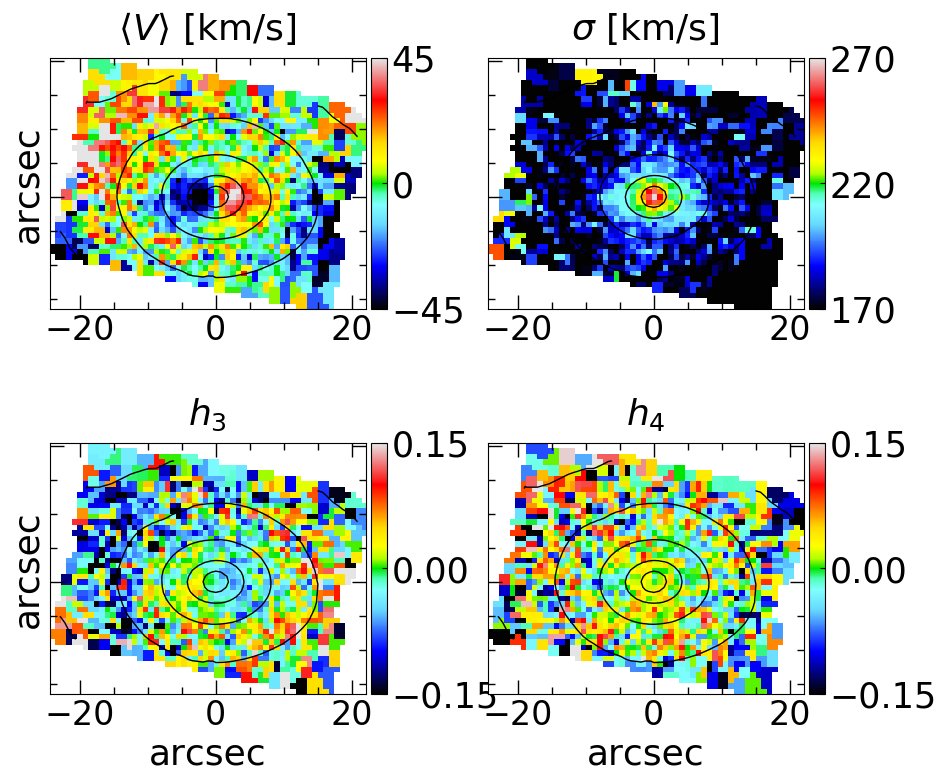
\includegraphics[width=\textwidth]{NGC3414_r6_voronoi.png}
		\caption{NGC 3414}
	\end{subfigure}
	\begin{subfigure}[b]{0.49\textwidth}
		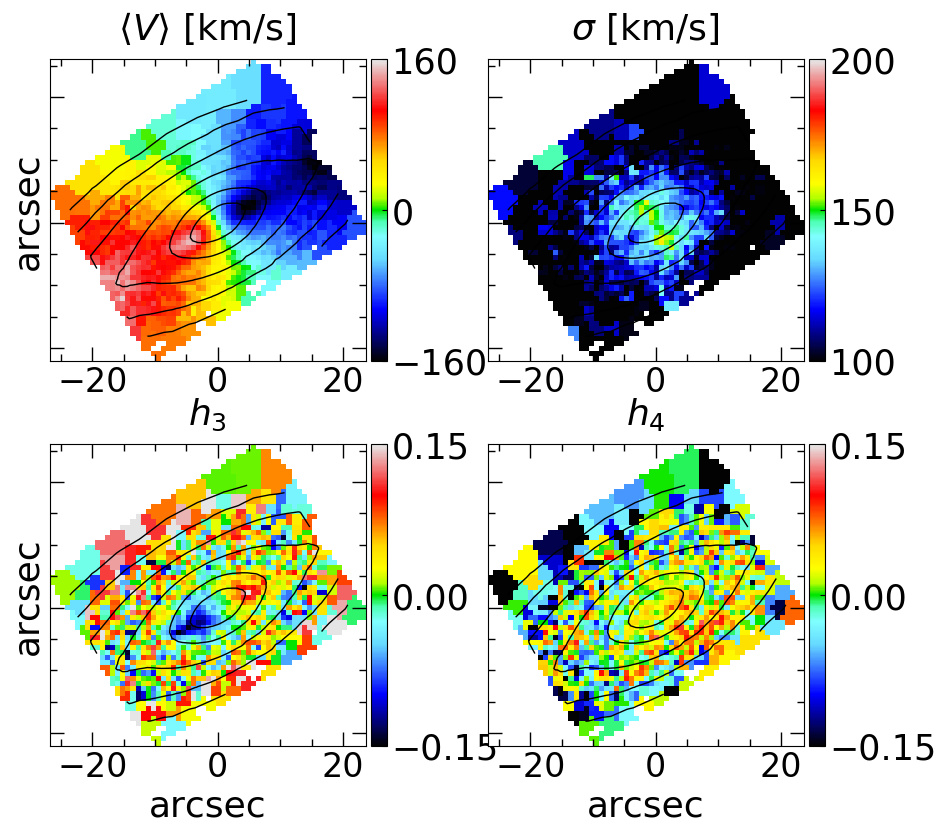
\includegraphics[width=\textwidth]{NGC4111_r1_voronoi.png}
		\caption{NGC 4111}
	\end{subfigure}
	\caption{IFU-maps of average LOS-velocities, velocity dispersion, $h_3$ parameters and $h_4$ parameters from two simulated merger remnants and two observed galaxies. The four maps in figure (a) are from the BH-0 merger, and the four in figure (b) are the BH-6 merger. Figures (c) and (d) show IFU-maps of known slow (NGC 3414) and fast rotator (NGC 4111) galaxies from the $\mathrm{ATLAS^{3D}}$ survey \citep{Emsellem2004, Cappellari2011}.}
	\label{figure:IFU-maps}
\end{figure}

Further analysis of the nature of the simulated mergers' rotation can be done by looking at the $\lambda_R$ parameter, which describes the angular momentum of a galaxy \citep{Emsellem2007}. More importantly, the parameter allows us to differentiate between the aforementioned slowly rotating galaxies and so-called fast rotators (see figure \ref{figure:IFU-maps}) \citep{Emsellem2007}. The parameter itself is defined in a general form as:
\begin{equation}
\lambda_R \equiv \frac{\langle R |V| \rangle}{\langle R \sqrt{V^2 + \sigma^2} \rangle}, \label{eq:general_lambdar}
\end{equation}
where $R$ is the projected distance from the galactic centre, $V$ is velocity, $\sigma$ is the velocity dispersion and $\langle \; \rangle$ denote that the nominator and denominator in the equation are luminosity weighted means. However, as most of the observational kinematic analysis of galaxies is done through binned 2D spectroscopy, and as the IFU-maps made from our simulations are produced the same way as the observed ones, we will be using the following version of the equation:
\begin{equation}
\lambda_R = \frac{\sum^{N_p}_{i=1} F_i R_i |V_i|}{\sum^{N_p}_{i=1} F_i R_i \sqrt{V_i^2 + \sigma^2_i}}, \label{eq:binned_lambdar}
\end{equation}
where $F_i$, $R_i$, $V_i$ and $\sigma_i$ are the flux, projected distance from the galaxy centre, velocity and velocity dispersion of the $i$th bin, and $N_p$ is the number of bins. In the case of our simulations, the $N_p$ bins used are of course the voronoi bins described earlier in this section. 

Determining whether a galaxy is either a fast or a slow rotator using $\lambda_R$, is done by comparing the value that the parameter gets at the galaxy's effective radius, to some pre-defined threshold. The originally used threshold is: $\lambda_{Re} < 0.1$, where $\lambda_{Re}$ is the aforementioned $\lambda_R$ at the effective radius, and where galaxies fulfilling the condition are classified as slow rotators \citep{Emsellem2007}. A revision of the threshold by \cite{Emsellem2011} takes the ellipticity ($\epsilon$) of the galaxy into account, and defines slow rotators as having $\lambda_{R_e} < 0.31 \sqrt{\epsilon}$, which accounts for the increased anisotropy in the kinematics of flatter galaxies. An even further refinement of the threshold has been proposed by \cite{Cappellari2016}, where slow rotator galaxies are determined using the following two criteria: $\lambda_{R_e} < 0.08 + \epsilon/4$ and $\epsilon < 0.4$. The former criterion of the threshold reduces the risk of misidentifying very round non-regular slow rotators as fast rotators, while the latter makes sure that only sufficiently round galaxies are classified as slow rotators (\cite{Cappellari2016} argues that "genuine" disk-less slow rotators are all rounder than $\epsilon = 0.4$).

Since two of the three aforementioned slow rotator thresholds require us to know the ellipticity of the galaxy, we calculate the simulated merger remnants' ellipticities before analysing their rotation. The ellipticity calculations are done using a method described in \cite{Zemp2011}, which uses the shape tensor:
\begin{equation}
\mathbf{S} = \frac{\int_V \rho(\mathbf{r}) \omega(\mathbf{r}) \mathbf{r} \mathbf{r}^T \; dV }{\int_V \rho{\mathbf{r}} \; dV},
\end{equation}
where $\mathbf{r}$ is position from the galactic centre, $\rho(\mathbf{r})$ is the mass density, $V$ is the volume of an enclosed ellipsoid with the elliptical radius $r_\mathrm{ell}$, and where the weighting function $\omega(\mathbf{r}) = 1$. The eigenvalues of the shape tensor correspond to $a^2/3$, $b^2/3$ and $c^2/3$; where $a$, $b$ and $c$ are the semi-principal axes; and which can be used to calculate the ellipticity as $\epsilon = 1 - b/a$. 

However, simply calculating the shape tensor and getting the correct eigenvalues is not possible, as the elliptical radius $r_\mathrm{ell}$ is defined, in part, by using the axis ratios $a/b$ and $a/c$:
\begin{equation}
r_\mathrm{ell} = \sqrt{x_\mathrm{ell}^2 + \frac{y_\mathrm{ell}^2}{(b/a)^2} + \frac{z_\mathrm{ell}^2}{(c/a)^2}}.
\end{equation}
This means that we have to turn the calculation into an iterative process by starting with $b/a = c/a = 1$ for the initial value of $r_\mathrm{ell}$, and calculating new shape tensor eigenvalues using previously gained axis ratios until the values of the ratios start to converge. 

We calculate $\lambda_{Re}$ and $\epsilon_e$, i.e. the ellipticity at the effective radius (the ellipticity is calculated using $r_\mathrm{ell} = R_e$, and a convergence criterion of a difference smaller than $10^{-3}$ between consequent axis ratios), for every merger simulation snapshot and plot them against each other. We also plot the previously mentioned slow rotator thresholds, as well as observations from the $\mathrm{ATLAS^{3D}}$-survey \citep{Cappellari2011}, in the same figure. The resulting plot can be seen in figure \ref{figure:lambda_epsilon}. 

\begin{figure}[h]
	\centering
	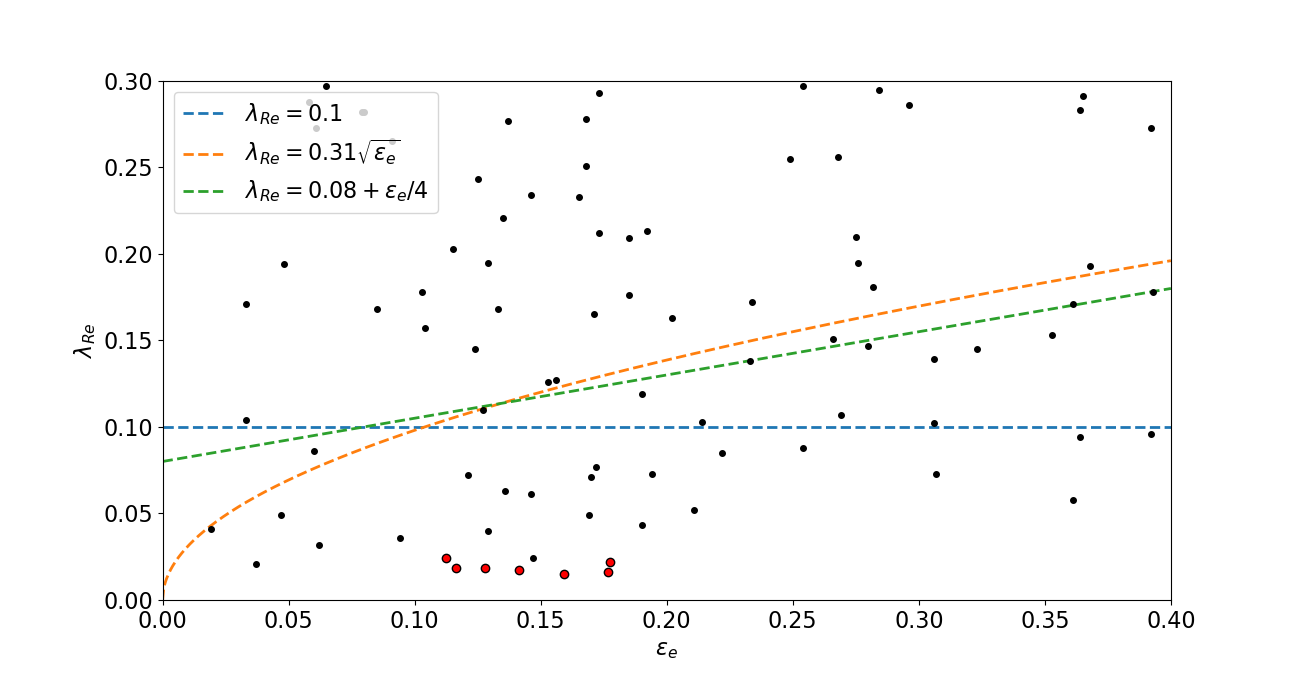
\includegraphics[width=\textwidth]{lambda_epsilon.png}
	\caption{The values of the $\lambda_{\mathrm{Re}}$-parameter of galaxies, plotted against their ellipticity at the effective radius. The red dots correspond to the simulated merger remnants, where as the black dots correspond to galaxies observed in the $\mathrm{ATLAS^{3D}}$-survey \citep{Cappellari2011, Emsellem2011}. The dashed lines display different slow rotator thresholds as a function of ellipticity \citep{Emsellem2007, Emsellem2011, Cappellari2016}.}
	\label{figure:lambda_epsilon}
\end{figure}

Regardless of the threshold used for differentiating between slow and fast rotators, figure \ref{figure:lambda_epsilon} shows us that, all of the simulated merger remnants are clearly classified as slow rotators. This agrees well with the kinematic anisotropies seen in the IFU maps, which also implied a slow rotator classification for the remnants.

\section{Comparison to NGC 1600}

As the physical properties of the merger progenitors are modelled after NGC 1600, it is interesting to see how the results from the simulations compare with actual observations of the galaxy. I am mainly comparing the observations to the BH-6 merger remnant, as the mass of the SMBH binary in the simulation is equivalent to the assumed mass of the central SMBH in NGC 1600 ($M_\bullet = 1.7 \times 10^{10} M_\odot$) \citep{Thomas2016}.

\begin{figure}
	\centering
	\begin{subfigure}[b]{0.49\textwidth}
		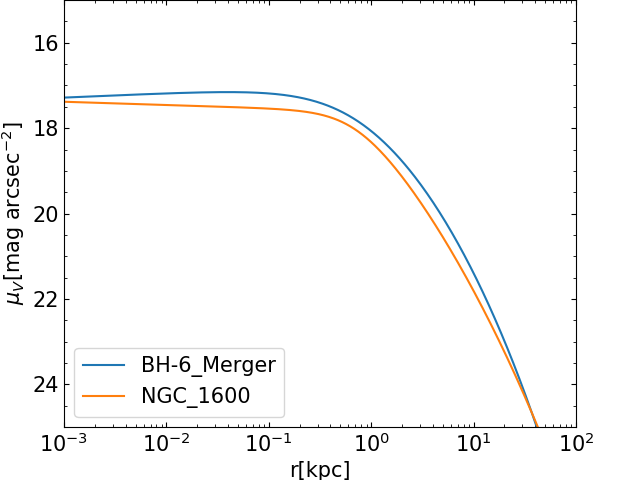
\includegraphics[width=\textwidth]{BH-6_NGC1600.png}
	\end{subfigure}
	\begin{subfigure}[b]{0.49\textwidth}
		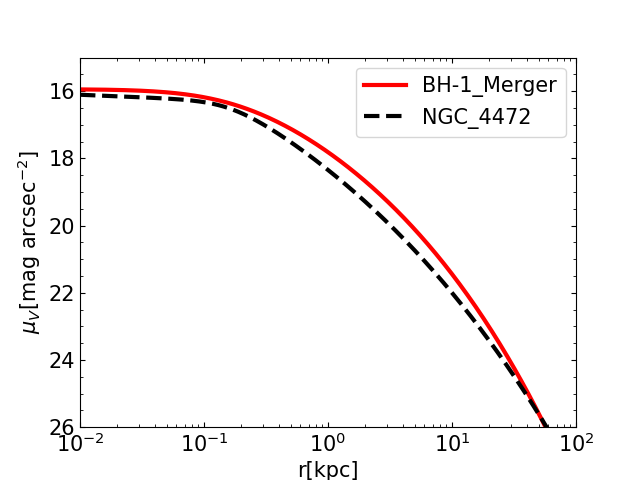
\includegraphics[width=\textwidth]{BH-1_NGC4472.png}
	\end{subfigure}
	\caption{Comparison between core-Sérsic profile fits from observed galaxies and simulated merger remnants. The figure on the left compares the profile of the BH-6 merger remnant (the merger remnant whose progenitors containing the largest central SMBH massess) to NGC 1600; while the figure on the right compares the profiles of the BH-1 merger remnant (the remnant with progenitors that had the smallest SMBH masses) and NGC 4472. The parameters for plotting the core-Sérsic profile of NGC 1600 were taken from \cite{Thomas2016}, with the units being changed to the above, by assuming $V - R = 0.5$ (the same assumption being done in \cite{Lauer2007}), and by using the distance $D = 64 \mathrm{Mpc}$ \citep{Thomas2016} to define the relation between arc seconds and parsecs. The parameters for the profile of NGC 4472 were from \cite{Dullo2012} and \cite{Lauer2007}.}
	\label{figure:profile_comparison}
\end{figure}

Figure \ref{figure:coresersic_sim_obs} shows the core-Sérsic profile fits of the surface brightness profiles alongside the best-fit parameters from Snapshot-6 and NGC 1600, as well as from Snapshot-1 and NGC 4472. Comparing the profiles of Snapshot-6 and NGC 1600, one can see unmistakeable similarities. Not only are the shapes of the profiles extremely similar, apart from the larger core and effective radii, the best-fit parameters are also quite closely related.

A further comparison between some of the properties of the two galaxies can be seen in table \ref{table:snap6_vs_NGC1600}. Most importantly the table shows that even their kinematic properties are alike, or in the very least, of the same order of magnitude. Furthermore, much like the merger remnants seen in the snapshots, by looking at it's $\lambda_e$ parameter and ellipticity at the effective radius, NGC 1600 can easily be identified as a slow rotator.

\begin{table}
	\begin{center}
		\scriptsize
		\begin{tabular}{c c c c c c c c c c}
		\hline
		\hline
		Galaxy & $M_\star$ & $M_\bullet$ & $R_e$ & $\mu_e$ & $n$ & 
		$V_\mathrm{LOS}$ & $\sigma_e$ & $\lambda_e$ &
		$\epsilon_e$ \\
		& $[\times 10^{11} M_\odot]$ & $[\times 10^{10} M_\odot]$ &
		[kpc] & [$\mathrm{mag/arcsec^2}$] & & [km/s] & [km/s] & & \\
		(1) & (2) & (3) & (4) & (5) & (6) & (7) & (8) & (9) & (10) \\
		\hline
		BH-6 merger & $8.3$ & $1.7$ & $8.914$ & $17.7$ & $4$ & $5.84$ & $311$ & $0.0215$ & $0.14$ \\
		NGC 1600 & $8.3$ & $1.7$ & $\sim 16$ & $\sim 22.8$ & $5.83$ & $3.4$ & 
		$293$ & $0.026$ & $0.32$ \\
		\hline
		\end{tabular}
	\end{center}
	\caption{Comparison between the physical properties of the simulated merger remnant BH-6 merger and the galaxy NGC 1600. The properties described in the columns are explained below, with the sources for the properties of NGC 1600 being written inside the brackets. \\
	(1) Name of the galaxy. \\
	(2) Total stellar mass \citep{Thomas2016}. \\
	(3) For SNapshot-6: central SMBH binary mass. For NGC 1600: central SMBH mass \citep{Thomas2016}. \\
	(4) Effective radius \citep{Thomas2016}. For NGC 1600, the effective radius is changed from arc seconds to kpc by assuming that it is located at the distance of $D = 64 \; \mathrm{Mpc}$ \citep{Thomas2016}. \\
	(5) Surface brightness at the effective radius. Calculated from the best fit core-Sérsic profile parameters given in \cite{Thomas2016}. \\
	(6) Sérsic index from the best fitting core-Sérsic profile fit \citep{Thomas2016}. \\
	(7) Mean line-of-sight velocity inside the effective radius \citep{Bender1994}. \\
	(8) Velocity dispersion inside the effective radius \citep{Veale2017veldisp}. For "Snapshot-6", the given velocity dispersion is calculated from a Voronoi binned image as the mean of the velocity dispersion values of the bins located inside the effective radius. \\
	(9) Spin parameter at the effective radius \citep{Veale2018lambda}. \\
	(10) For BH-6 merger: ellipticity of the galaxy at the effective radius; and for NGC 1600: luminosity weighted ellipticity \citep{Goullaud2018}.
	}
	\label{table:snap6_vs_NGC1600}
\end{table}

Of course, due to the nature in which the merger progenitors were modelled, the physical parameters being similar between the simulated merger remnant and NGC 1600 isn't unexpected. This result does however further imply that the light deficiency observed in the cores of galaxies such as NGC 1600 is formed similarly to the simulations, i.e. through a scouring process caused by a binary SMBH during a galaxy merger.


\chapter{Conclusions}

\appendix

\chapter{Figures}

\begin{figure}
	\centering
	\begin{subfigure}[b]{0.49\textwidth}
		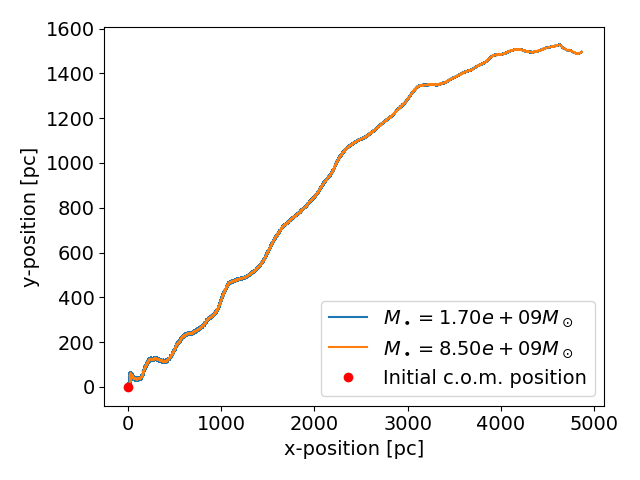
\includegraphics[width=\textwidth]{Run1_Trajectory_small.png}
		\caption{Run 1}
	\end{subfigure}
	\begin{subfigure}[b]{0.49\textwidth}
		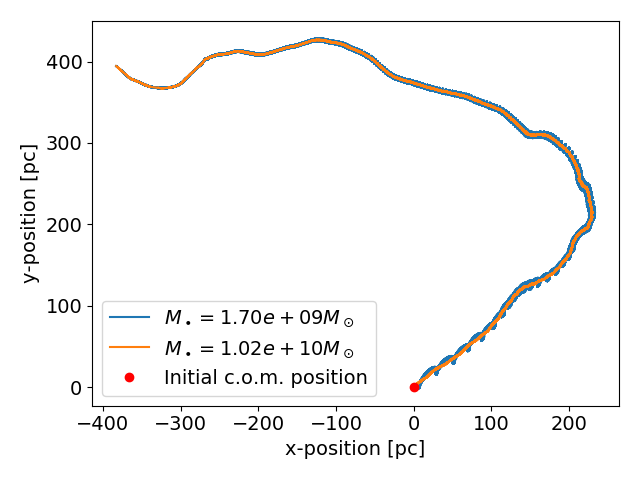
\includegraphics[width=\textwidth]{Run2_Trajectory_small.png}
		\caption{Run 2}
	\end{subfigure}
	\begin{subfigure}[b]{0.49\textwidth}
		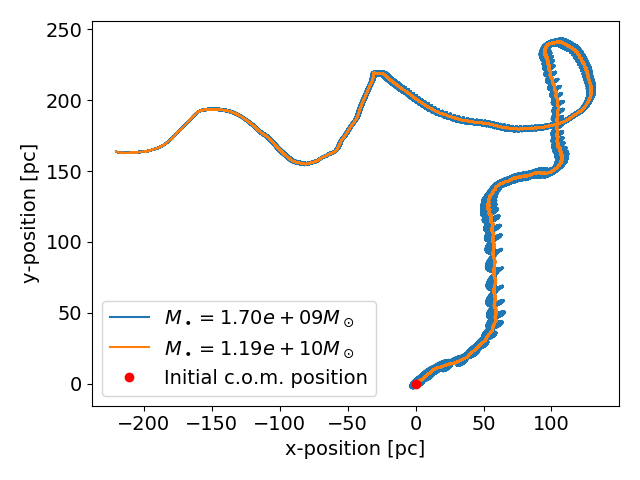
\includegraphics[width=\textwidth]{Run3_Trajectory_small.png}
		\caption{Run 3}
	\end{subfigure}
	\begin{subfigure}[b]{0.49\textwidth}
		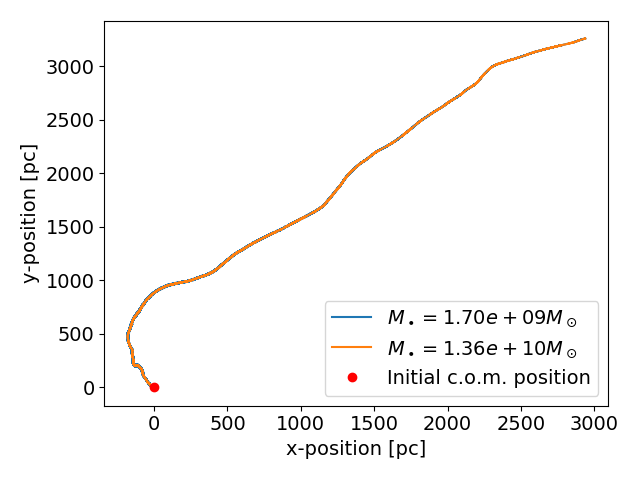
\includegraphics[width=\textwidth]{Run4_Trajectory_small.png}
		\caption{Run 4}
	\end{subfigure}
	\caption{The trajectories of the black holes from simulation runs by \cite{Mannerkoski2019}. The coordinates are centred on the initial location of the centre-of-mass of the black hole system. The orange and blue lines show the paths taken by the smaller and larger black holes respectively during the simulation.}
	\label{figure:all_traj}
\end{figure}

\begin{figure}[h]
	\centering
	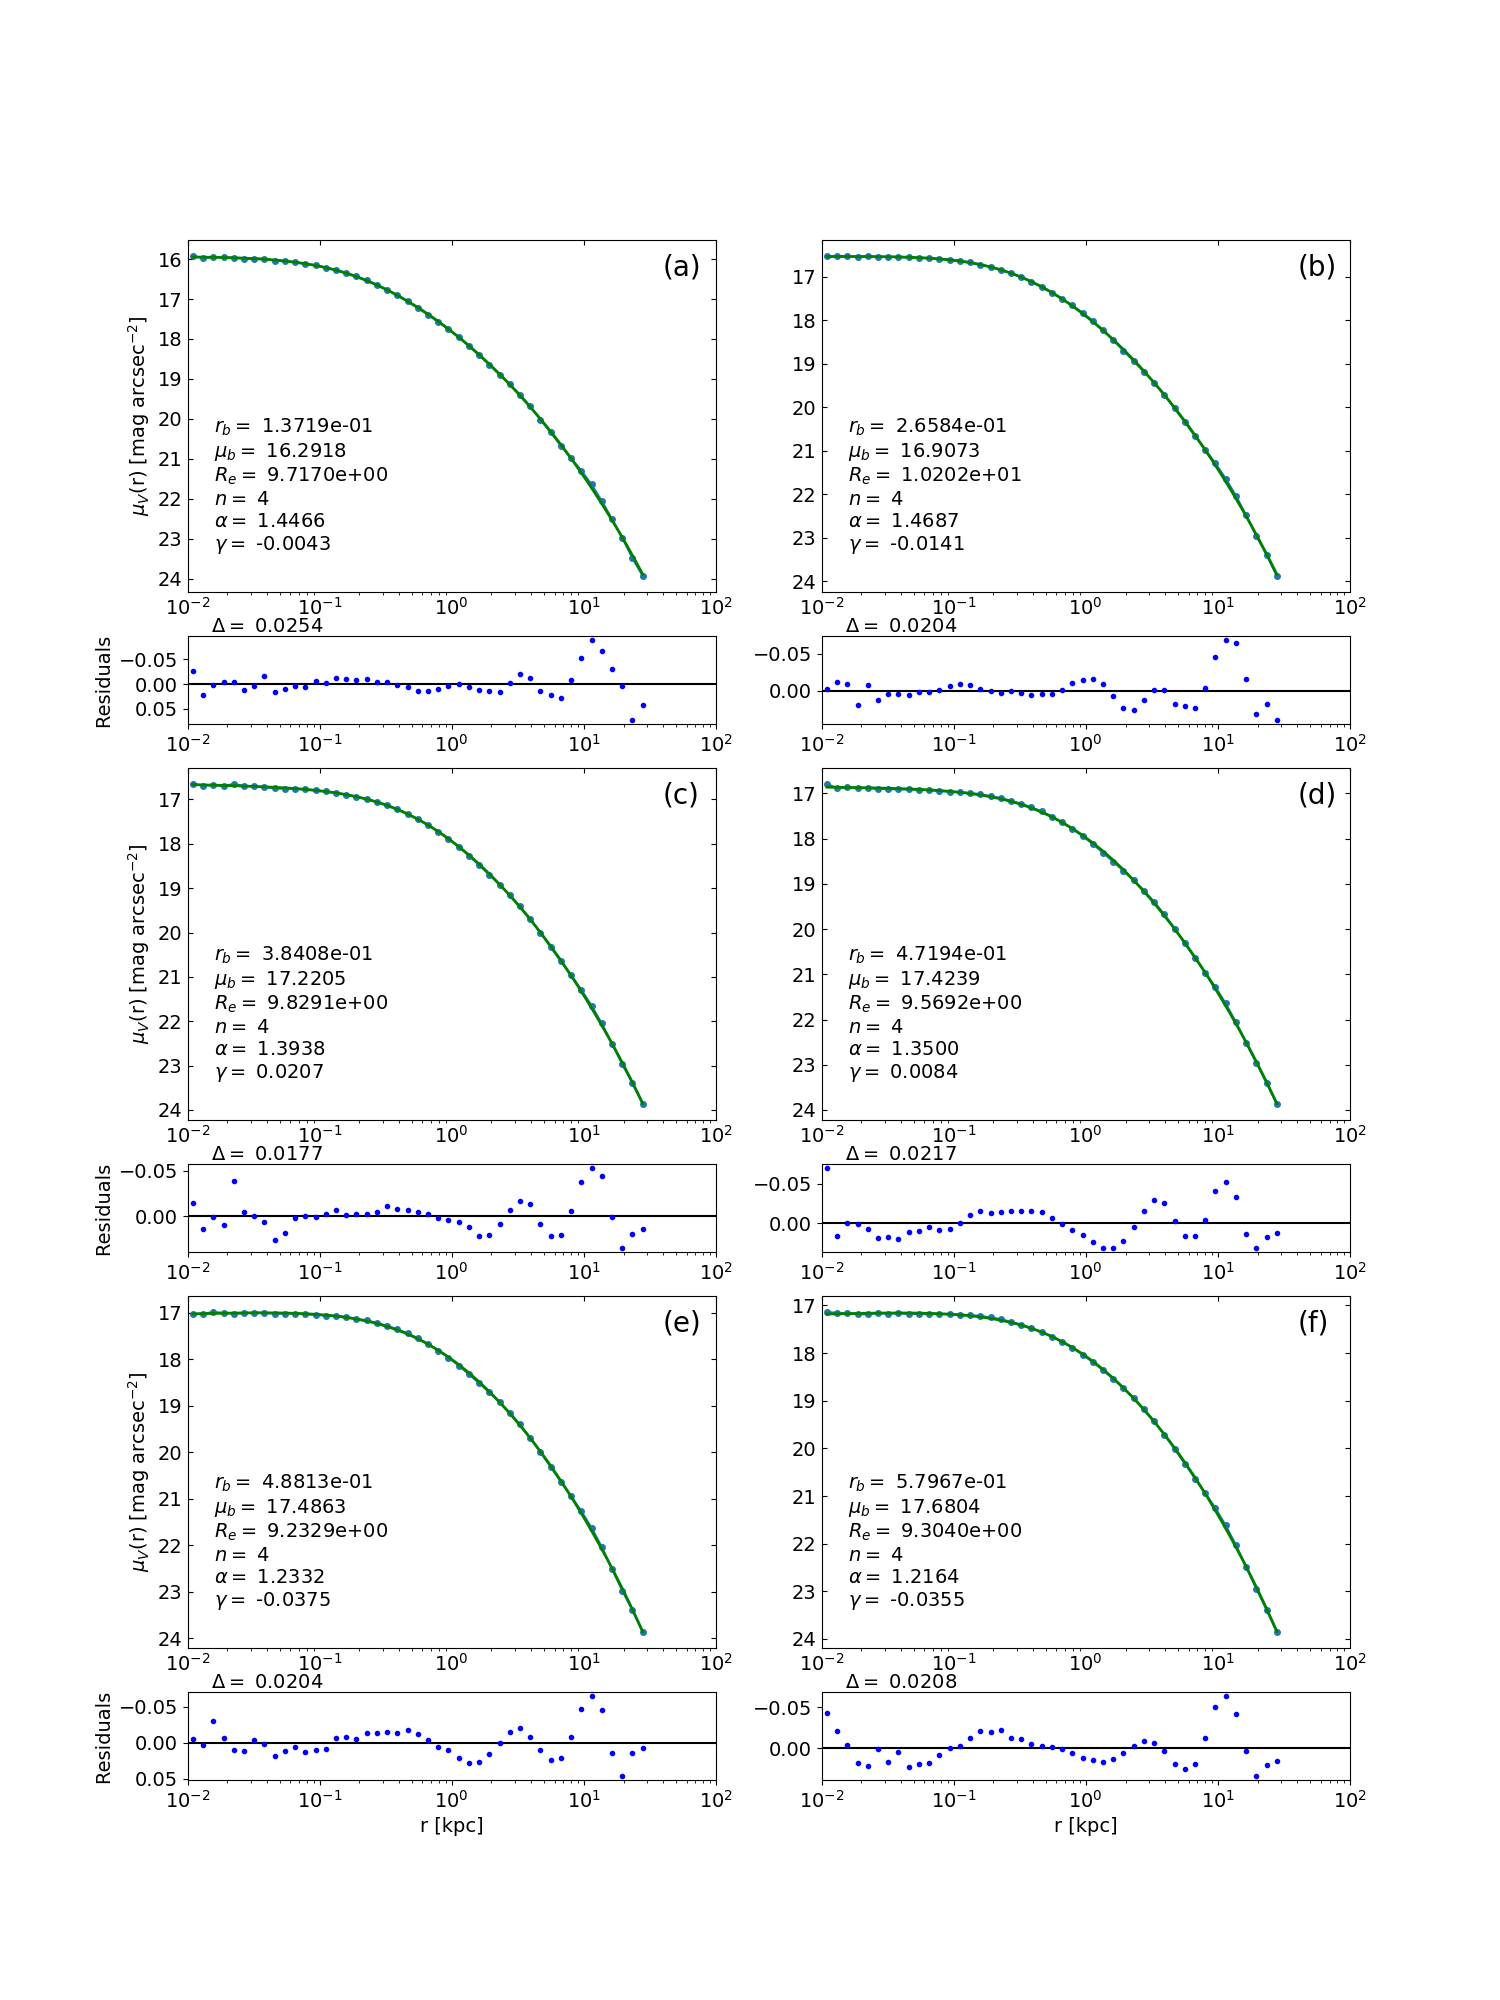
\includegraphics[width=\textwidth]{all_core_profiles.png}
	\caption{Core-Sérsic profile fits of the surface brightness data calculated from all of the individual simulated merger remnants with progenitors containing central supermassive black holes. The letters (a)-(f) denote the different snapshots ((a): BH-1 merger, (b): BH-2 merger, (c): BH-3 merger, (d): BH-4 merger, (e): BH-5 merger, (f): BH-6 merger).}
	\label{figure:all_core}
\end{figure}

\begin{figure}[h]
	\centering
	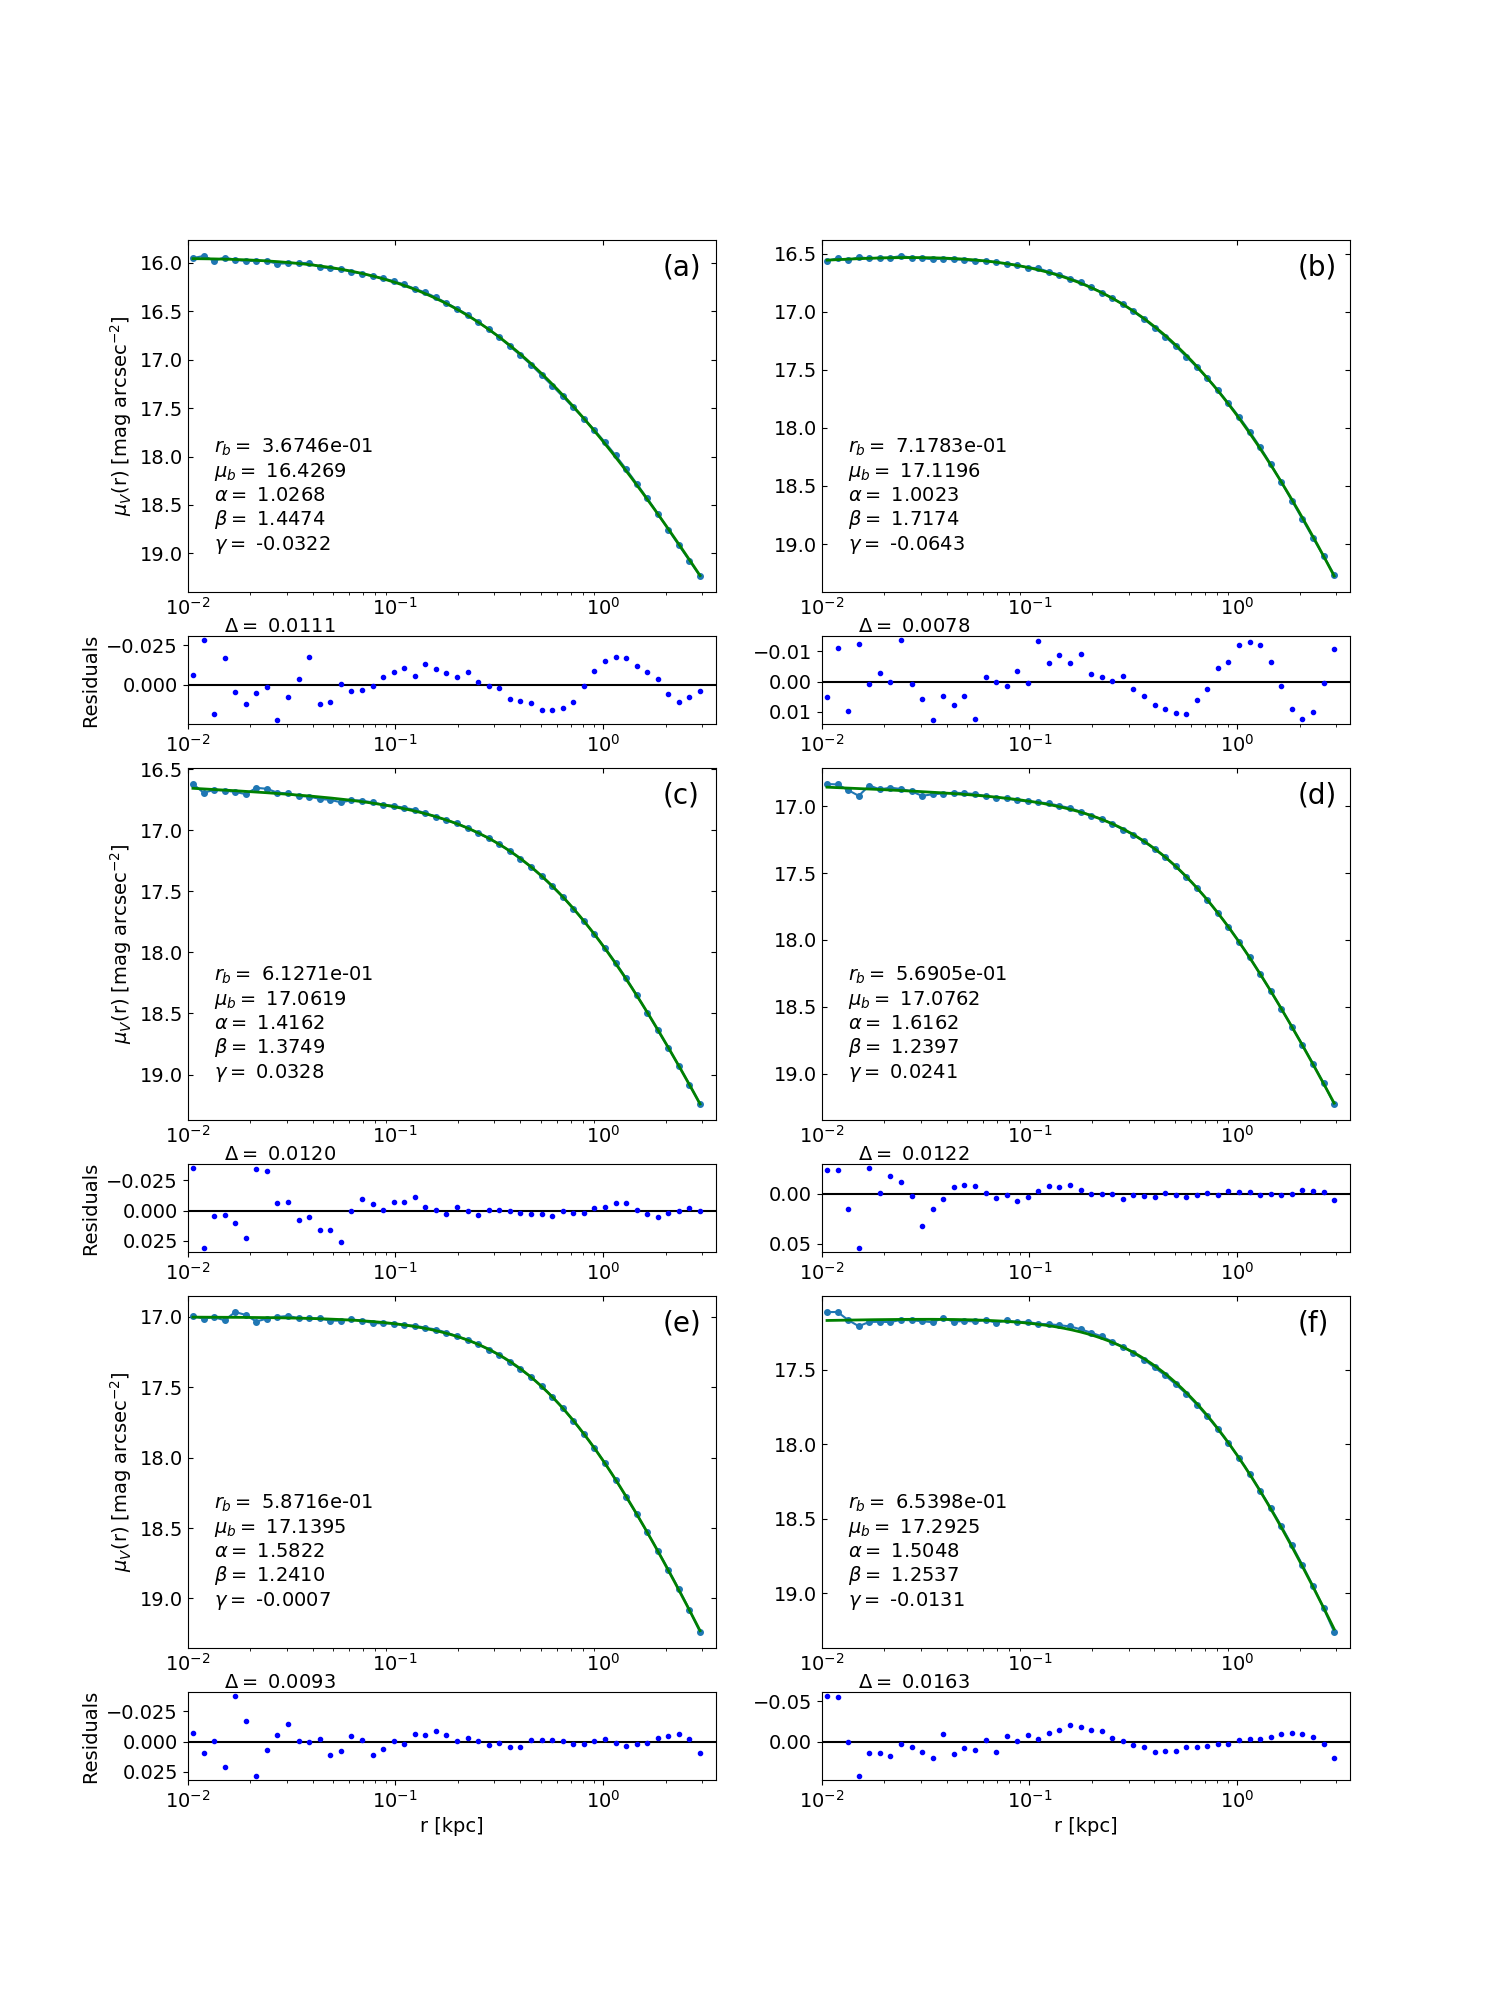
\includegraphics[width=\textwidth]{all_nuker_profiles.png}
	\caption{Nuker profile fits of the surface brightness data calculated from all of the individual simulated merger remnants with progenitors containing central supermassive black holes. The letters (a)-(f) denote the different merger remnants ((a): BH-1 merger, (b): BH-2 merger, (c): BH-3 merger, (d): BH-4 merger, (e): BH-5 merger, (f): BH-6 merger).}
	\label{figure:all_nuker}
\end{figure}

\begin{figure}
	\centering
	\begin{subfigure}[b]{0.49\textwidth}
		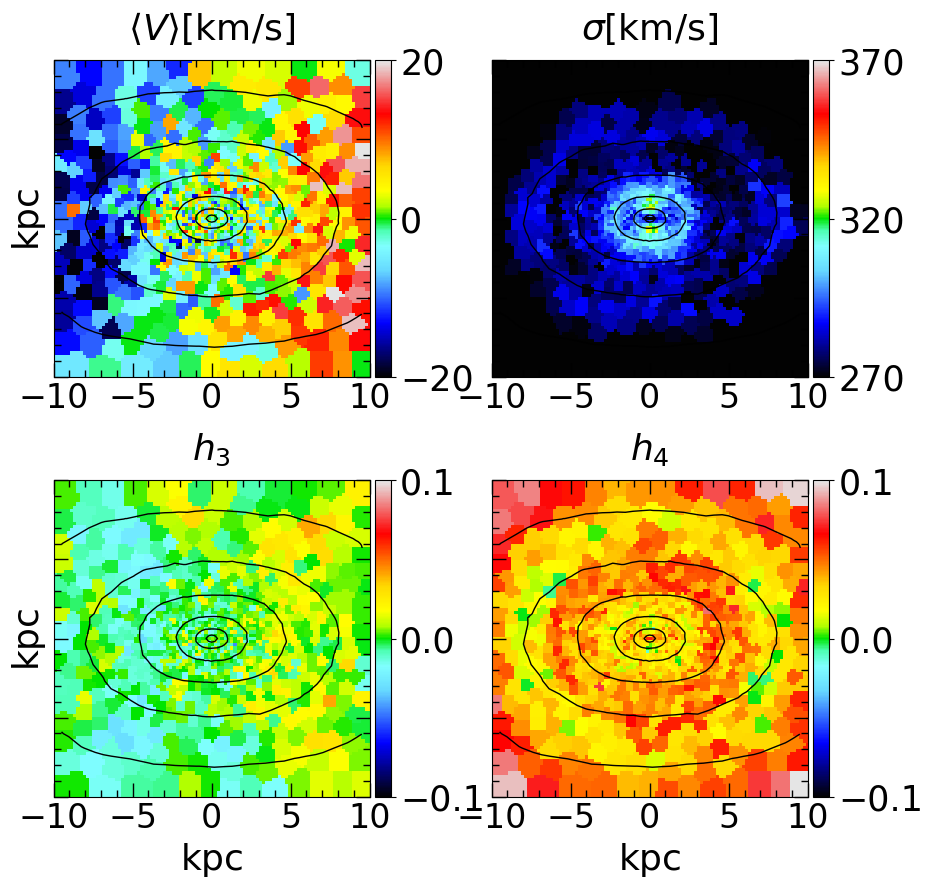
\includegraphics[width=\textwidth]{BH_0.png}
		\caption{BH-0 merger}
	\end{subfigure}
	\begin{subfigure}[b]{0.49\textwidth}
		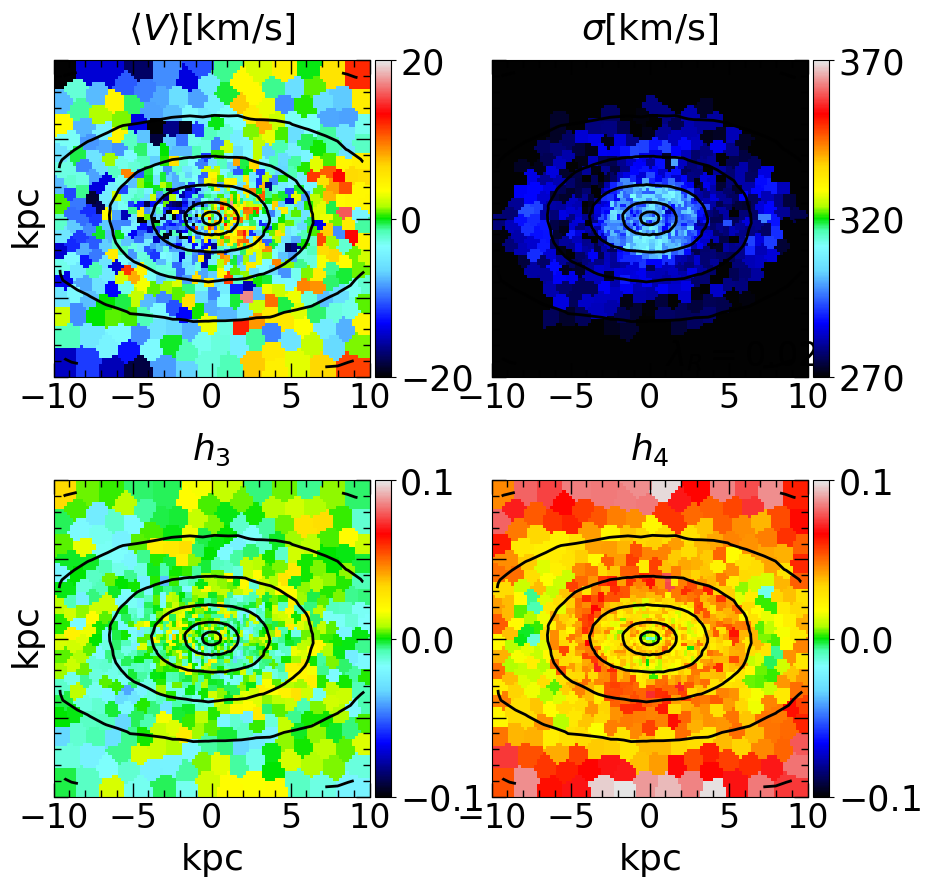
\includegraphics[width=\textwidth]{BH_1.png}
		\caption{BH-1 merger}
	\end{subfigure}
	\begin{subfigure}[b]{0.49\textwidth}
		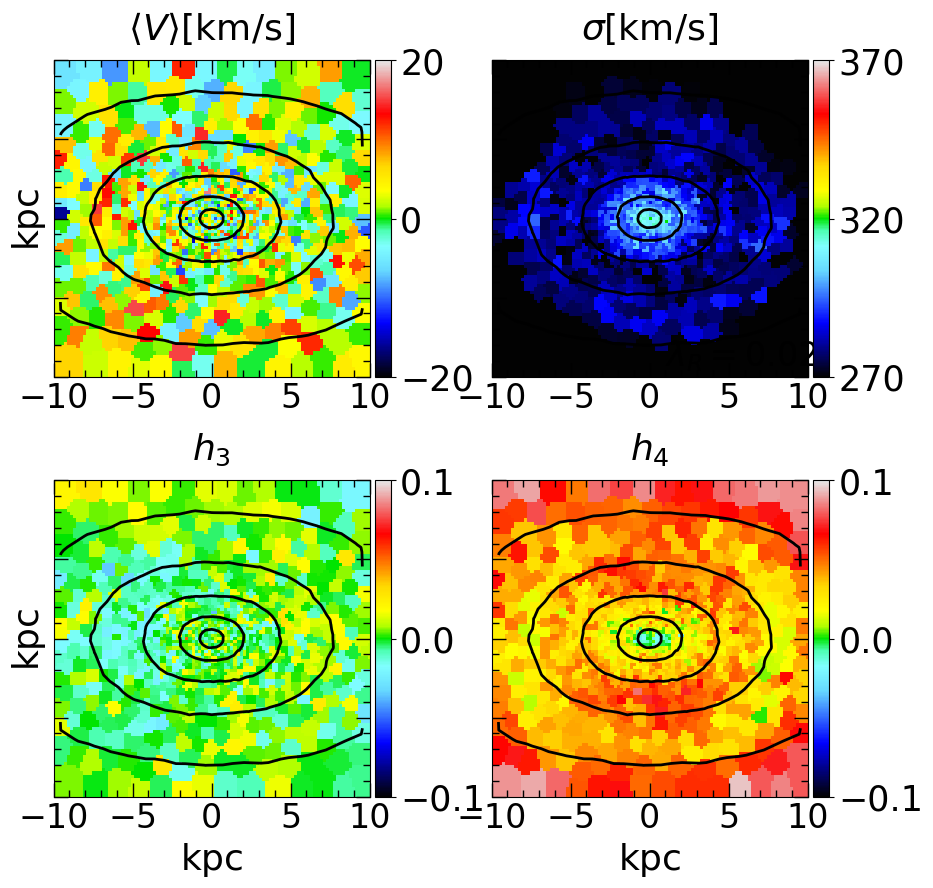
\includegraphics[width=\textwidth]{BH_2.png}
		\caption{BH-2 merger}
	\end{subfigure}
	\begin{subfigure}[b]{0.49\textwidth}
		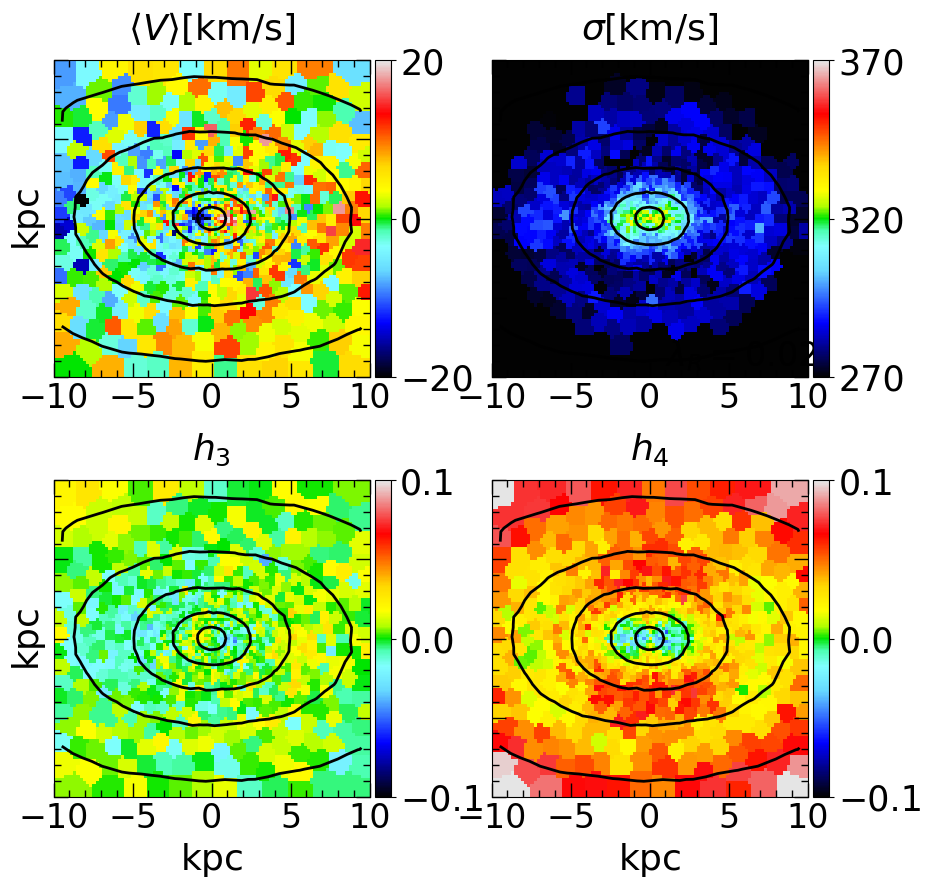
\includegraphics[width=\textwidth]{BH_3.png}
		\caption{BH-3 merger}
	\end{subfigure}
	\caption{IFU-maps of average LOS-velocities, velocity dispersion, $h_3$ parameters and $h_4$ parameters from four simulated merger remnants: Snapshot-0, Snapshot-1, Snapshot-2 and Snapshot-3.}
	\label{figure:all_voronoi_1}
\end{figure}

\begin{figure}
	\centering
	\begin{subfigure}[b]{0.49\textwidth}
		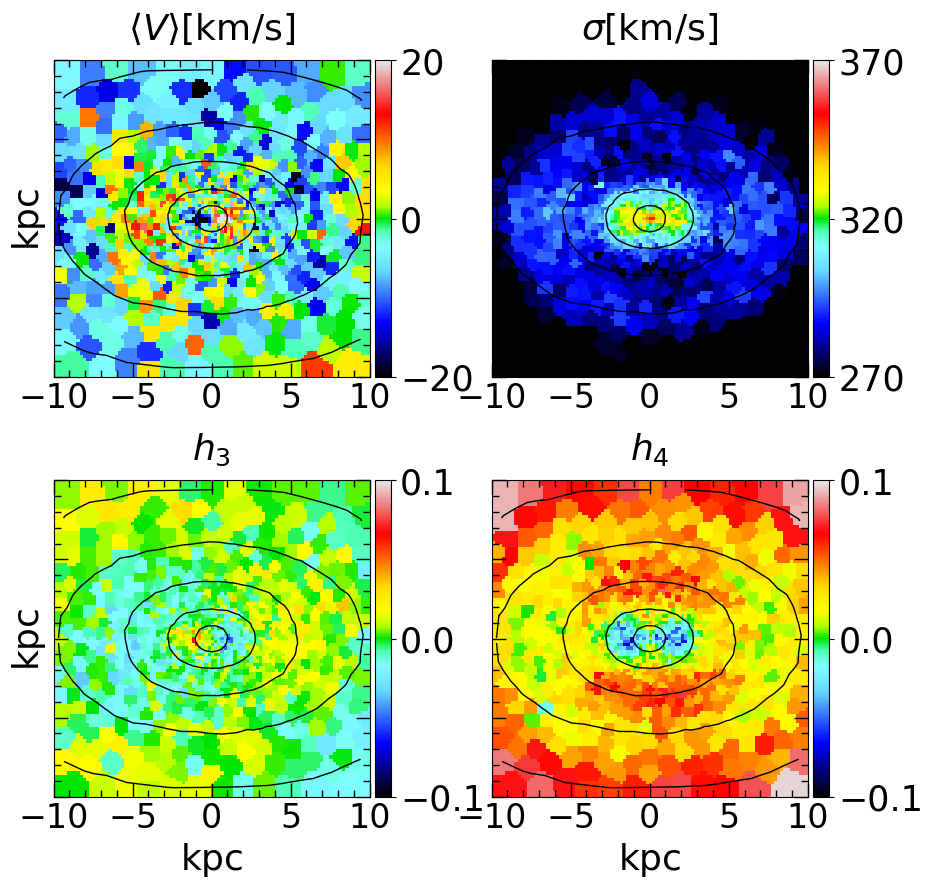
\includegraphics[width=\textwidth]{BH_4.png}
		\caption{BH-4 merger}
	\end{subfigure}
	\begin{subfigure}[b]{0.49\textwidth}
		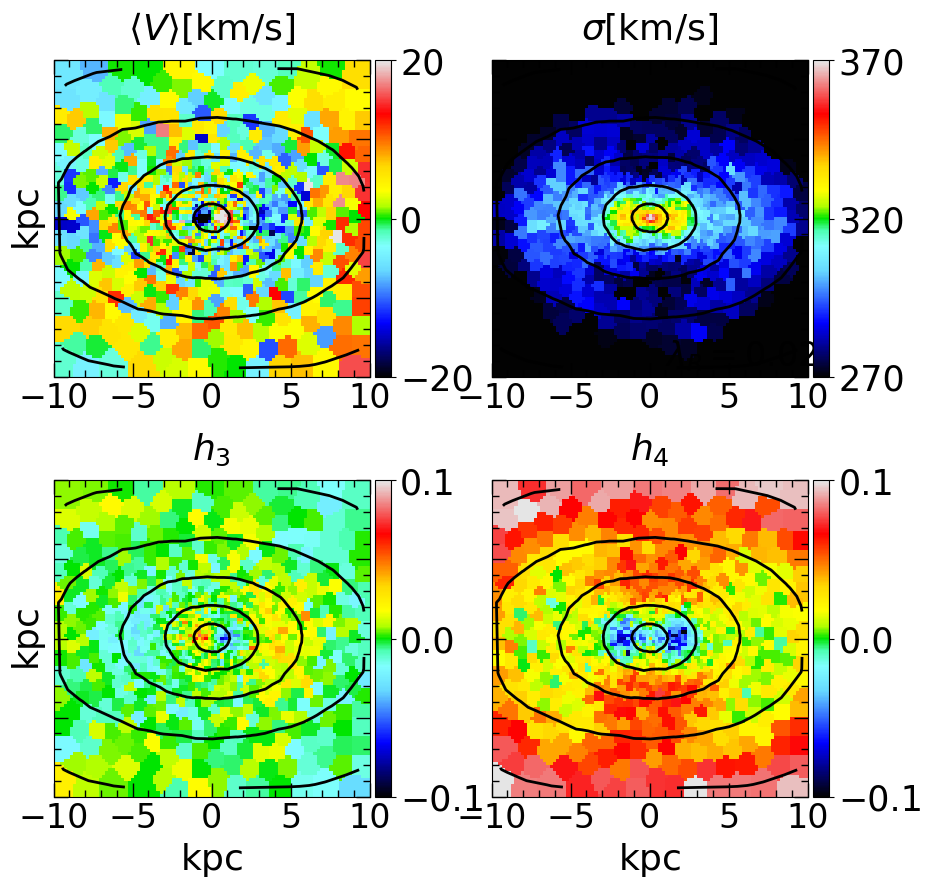
\includegraphics[width=\textwidth]{BH_5.png}
		\caption{BH-5 merger}
	\end{subfigure}
	\begin{subfigure}[b]{0.49\textwidth}
		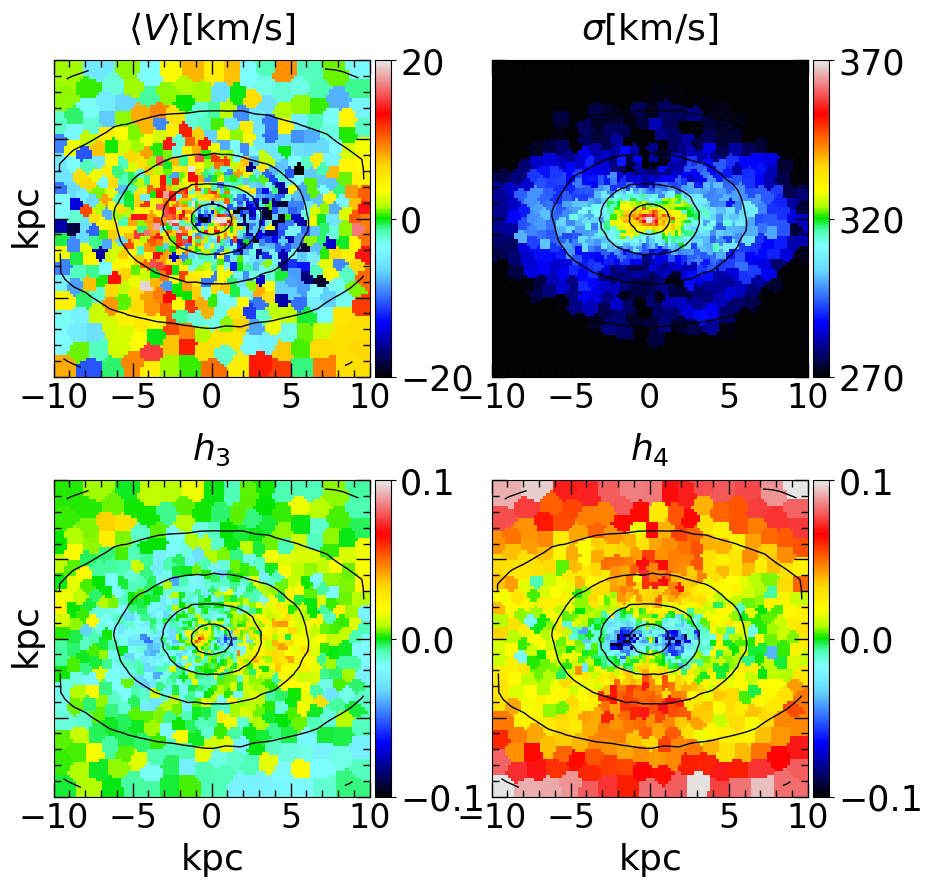
\includegraphics[width=\textwidth]{BH_6.png}
		\caption{BH-6 merger}
	\end{subfigure}
	\caption{IFU-maps of average LOS-velocities, velocity dispersion, $h_3$ parameters and $h_4$ parameters from three simulated merger remnants: Snapshot-4, Snapshot-5 and Snapshot-6.}
	\label{figure:all_voronoi_2}
\end{figure}

% STEP 5:
% Uncomment the following lines and set your .bib file and desired bibliography style
% to make a bibliography with BibTeX.
% Alternatively you can use the thebibliography environment if you want to add all
% references by hand.


% Define journal names
\newcommand{\apj}{The Astrophysical Journal}
\newcommand{\mnras}{Monthly Notices of the Royal Astronomical Society}
\newcommand{\apjs}{The Astrophysical Journal Supplement}
\newcommand{\nat}{Nature}
\newcommand{\aj}{The Astronomical Journal}
\newcommand{\na}{New Astronomy}
\newcommand{\araa}{Annual Review of Astronomy and Astrophysics}

\clearpage
\addcontentsline{toc}{chapter}{Bibliography} % This lines adds the bibliography to the ToC
\bibliographystyle{plainnat}
\bibliography{bibliography.bib}


\end{document}

